\newpage
\appendix
\renewcommand{\appendixname}{Apéndice}

\newpage
\cleardoublepage % Limpia cualquier residuo de contadores anteriores
\refstepcounter{section}
\def\thesection{A} % <--- ¡ESTO SOLUCIONA EL ERROR! Fuerza a que el valor de la referencia sea solo "A"
\label{anexo:pids}
\begin{center}
	\bfseries Apéndice A \\
	\normalfont\bfseries\itshape PIDs OBD-II Modo 01 — Datos en Tiempo Real
\end{center}
\addcontentsline{toc}{section}{Apéndice A: PIDs OBD-II Modo 01}

\vspace{4mm}

% --- CONFIGURACIÓN DE ENCABEZADOS PARA TABLAS LARGAS ---
\small
\renewcommand{\arraystretch}{1.3}
\tablefirsthead{
	\multicolumn{6}{l}{\textbf{Tabla A1} \textit{Códigos de Parámetro (PIDs) del Modo 01 del estándar OBD-II.}} \\ \toprule
	\textbf{PID (hex)} & \textbf{Bytes} & \textbf{Descripción} & \textbf{Mín.} & \textbf{Máx.} & \textbf{Unidad} \\ \midrule
}
\tablehead{
	\multicolumn{6}{l}{\textit{Continúa de la página anterior...}} \\ \toprule
	\textbf{PID (hex)} & \textbf{Bytes} & \textbf{Descripción} & \textbf{Mín.} & \textbf{Máx.} & \textbf{Unidad} \\ \midrule
}
\tabletail{\hline \multicolumn{6}{r}{\textit{Continúa en la siguiente página...}} \\}
\tablelasttail{\bottomrule}

% --- CUERPO DE LA TABLA QUE CAMBIA DE HOJA AUTOMÁTICAMENTE ---
\begin{supertabular}{ccp{7cm}ccc}
	00 & 4 & PIDs implementados [01--20] & -- & -- & bits \\
	01 & 4 & Estado de monitores de diagnóstico (MIL y DTC) & -- & -- & bits \\
	02 & 2 & Código de falla DTC almacenado & -- & -- & bits \\
	03 & 2 & Estado del sistema de combustible & -- & -- & bits \\
	04 & 1 & Carga calculada del motor & 0 & 100 & \% \\
	05 & 1 & Temperatura del líquido de enfriamiento & -40 & 215 & °C \\
	06 & 1 & Ajuste de combustible corto plazo — Banco 1 & -100 & 99.2 & \% \\
	07 & 1 & Ajuste de combustible largo plazo — Banco 1 & -100 & 99.2 & \% \\
	08 & 1 & Ajuste de combustible corto plazo — Banco 2 & -100 & 99.2 & \% \\
	09 & 1 & Ajuste de combustible largo plazo — Banco 2 & -100 & 99.2 & \% \\
	0A & 1 & Presión del combustible & 0 & 765 & kPa \\
	0B & 1 & Presión absoluta del colector de admisión & 0 & 255 & kPa \\
	0C & 2 & RPM del motor & 0 & 16383.75 & rpm \\
	0D & 1 & Velocidad del vehículo & 0 & 255 & km/h \\
	0E & 1 & Avance del tiempo de encendido & -64 & 63.5 & ° \\
	0F & 1 & Temperatura del aire de admisión & -40 & 215 & °C \\
	10 & 2 & Velocidad de flujo de aire MAF & 0 & 655.35 & g/s \\
	11 & 1 & Posición del acelerador & 0 & 100 & \% \\
	12 & 1 & Estado del aire secundario & -- & -- & bits \\
	1C & 1 & Estándar OBD implementado & -- & -- & bits \\
	1F & 2 & Tiempo desde arranque del motor & 0 & 65535 & s \\
	21 & 2 & Distancia recorrida con MIL encendido & 0 & 65535 & km \\
	2C & 1 & EGR comandado & 0 & 100 & \% \\
	2F & 1 & Nivel del tanque de combustible & 0 & 100 & \% \\
	31 & 2 & Distancia recorrida desde borrado de fallas & 0 & 65535 & km \\
	33 & 1 & Presión barométrica absoluta & 0 & 255 & kPa \\
	3C & 2 & Temperatura del catalizador: Banco 1, Sensor 1 & -40 & 6513.5 & °C \\
	42 & 2 & Voltaje del módulo de control & 0 & 65.535 & V \\
	45 & 1 & Posición relativa del acelerador & 0 & 100 & \% \\
	46 & 1 & Temperatura del aire ambiental & -40 & 215 & °C \\
	4D & 2 & Tiempo con MIL encendido & 0 & 65535 & min \\
	5A & 1 & Posición relativa del pedal del acelerador & 0 & 100 & \% \\
	5C & 1 & Temperatura del aceite del motor & -40 & 210 & °C \\
	5E & 2 & Velocidad del combustible del motor & 0 & 3276.75 & L/h \\
	61 & 1 & Porcentaje de torque solicitado por conductor & -125 & 125 & \% \\
	62 & 1 & Porcentaje de torque actual del motor & -125 & 125 & \% \\
	63 & 2 & Torque de referencia del motor & 0 & 65535 & Nm \\
\end{supertabular}

\vspace{3mm}

	\textit{Nota.} Selección de los PIDs más relevantes del Modo 01 del estándar OBD-II, correspondientes a datos en tiempo real provistos por la ECU del vehículo. La lista completa incluye PIDs adicionales hasta el código \texttt{C4}. Adaptado de \textit{El OBDII Completo/Los PIDs/PID Modo 01}, por Wikilibros, 2024 (\url{https://es.wikibooks.org/wiki/El_OBDII_Completo/Los_PIDs/PID_Modo_01}). Contenido bajo licencia Creative Commons Atribución-CompartirIgual.


\newpage
\cleardoublepage % Limpia cualquier residuo de contadores anteriores
\refstepcounter{section}
\def\thesection{B} % <--- Fuerza a que el valor de la referencia sea solo "B"
\label{anexo:tja1050}
\begin{center}
	\bfseries Apéndice B \\
	\normalfont\bfseries\itshape Hoja de Datos Técnicos del Transceptor CAN TJA1050
\end{center}
\addcontentsline{toc}{section}{Apéndice B: Hoja de Datos Técnicos del Transceptor CAN TJA1050}

\vspace{4mm}

El transceptor TJA1050 es la interfaz física entre el controlador del protocolo Area Network (CAN) y el bus físico diferencial de datos \citep{tja1050_datasheet}. Está diseñado específicamente para aplicaciones automotrices de alta velocidad que requieren tasas de transferencia de hasta 1~Mbaud.

\subsection*{Características Principales y Funcionalidades}
De acuerdo con las especificaciones del fabricante, el dispositivo destaca por las siguientes prestaciones de ingeniería:
\begin{itemize}
	\item \textbf{Compatibilidad Estándar:} Totalmente compatible con la norma internacional ISO 11898.
	\item \textbf{Inmunidad Electromagnética:} Emisión electromagnética (EME) extremadamente baja gracias al emparejamiento óptimo de las señales de salida CANH y CANL, combinada con una alta inmunidad a interferencias (EMI).
	\item \textbf{Compatibilidad Lógica:} Niveles de entrada tolerantes y compatibles con dispositivos de lógica de 5~V.
	\item \textbf{Protección Automotriz:} Pines de bus protegidos contra transitorios eléctricos en entornos automotrices de acuerdo con la norma ISO 7637, además de contar con protección térmica y salvaguarda contra cortocircuitos a batería y a masa.
	\item \textbf{Temporizador de Seguridad:} Circuito de tiempo muerto (\textit{Dominant Time-out}) en la línea TXD que previene el bloqueo permanente del bus por fallas de hardware.
\end{itemize}

\subsection*{Configuración de Pines (Pinout)}
El TJA1050 se presenta en un encapsulado plástico de contorno reducido SO8 con 8 terminales. La función de cada pin se detalla a continuación en la Tabla B1.

\vspace{2mm}

% --- CONFIGURACIÓN DE ENCABEZADOS PARA TABLA B1 (3 COLUMNAS) ---
\small
\renewcommand{\arraystretch}{1.3}
\tablefirsthead{
	\multicolumn{3}{l}{\textbf{Tabla B1} \textit{Descripción de pines del transceptor TJA1050.}} \\ \toprule
	\rowcolor{gray!15} \textbf{Símbolo} & \textbf{Pin} & \textbf{Descripción Técnica} \\ \midrule
}
\tablehead{
	\multicolumn{3}{l}{\textit{Tabla B1. Continúa de la página anterior...}} \\ \toprule
	\rowcolor{gray!15} \textbf{Símbolo} & \textbf{Pin} & \textbf{Descripción Técnica} \\ \midrule
}
\tabletail{\hline \multicolumn{3}{r}{\textit{Continúa en la siguiente página...}} \\}
\tablelasttail{\bottomrule}

\begin{center}
	\begin{supertabular}{p{1.5cm} p{1.5cm} p{10.5cm}}
		TXD  & 1 & Entrada de datos de transmisión; lee los datos lógicos provenientes del controlador CAN. \\ 
		GND  & 2 & Conexión de referencia a tierra (0~V). \\ 
		VCC  & 3 & Voltaje de alimentación principal (4.75~V a 5.25~V). \\ 
		RXD  & 4 & Salida de datos de recepción; envía los datos leídos desde el bus hacia el controlador CAN. \\ 
		Vref & 5 & Salida de voltaje de referencia del circuito ($0.5 \cdot V_{CC}$ nominal). \\
		CANL & 6 & Línea de nivel bajo del bus CAN físico (\textit{LOW-level CAN bus line}). \\ 
		CANH & 7 & Línea de nivel alto del bus CAN físico (\textit{HIGH-level CAN bus line}). \\ 
		S    & 8 & Entrada de selección de modo: conectar a GND para modo de alta velocidad o a VCC para modo silencioso. \\ 
	\end{supertabular}
\end{center}

{\raggedright\small\textit{Nota.} Datos técnicos adaptados de la especificación de producto de Philips Semiconductors para el encapsulado plástico SO8. Los pines lógicos de entrada (TXD y S) cuentan con tolerancia de nivel tanto para 3.3~V como para 5~V, facilitando el acoplamiento directo con el microcontrolador.\par}

\vspace{2mm}
\subsection*{Especificaciones Eléctricas de Referencia}
La Tabla B2 resume las magnitudes límites y de operación indispensables para el correcto acoplamiento eléctrico del componente dentro del hardware diseñado.

\vspace{2mm}

% --- CONFIGURACIÓN DE ENCABEZADOS PARA TABLA B2 (5 COLUMNAS) ---
\small
\renewcommand{\arraystretch}{1.3}
\tablefirsthead{
	\multicolumn{5}{l}{\textbf{Tabla B2} \textit{Valores eléctricos fundamentales y límites absolutos del TJA1050.}} \\ \toprule
	\rowcolor{gray!15} \textbf{Símbolo} & \textbf{Parámetro} & \textbf{Mínimo} & \textbf{Máximo} & \textbf{Unidad} \\ \midrule
}
\tablehead{
	\multicolumn{5}{l}{\textit{Tabla B2. Continúa de la página anterior...}} \\ \toprule
	\rowcolor{gray!15} \textbf{Símbolo} & \textbf{Parámetro} & \textbf{Mínimo} & \textbf{Máximo} & \textbf{Unidad} \\ \midrule
}
\tabletail{\hline \multicolumn{5}{r}{\textit{Continúa en la siguiente página...}} \\}
\tablelasttail{\bottomrule}

\begin{center}
	\begin{supertabular}{p{2.2cm} p{5.3cm} p{2.0cm} p{2.0cm} p{1.5cm}}
		$V_{CC}$ & Voltaje de alimentación de operación & 4.75 & 5.25 & V \\ 
		$V_{CC(abs)}$ & Voltaje de alimentación límite absoluto & -0.3 & +6.0 & V \\ 
		$V_{CANH}$ & Voltaje continuo en pin CANH & -27 & +40 & V \\ 
		$V_{CANL}$ & Voltaje continuo en pin CANL & -27 & +40 & V \\ 
		$V_{i(dif)(bus)}$ & Voltaje de entrada diferencial (Dominante) & 1.5 & 3.0 & V \\ 
		$t_{d(TXD-RXD)}$ & Retraso de propagación total (TXD a RXD) & — & 250 & ns \\
		$T_{vj}$ & Temperatura de unión virtual de operación & -40 & +150 & °C \\ 
		$V_{esd}$ & Voltaje de descarga electroestática (HBM) & -4000 & +4000 & V \\
	\end{supertabular}
\end{center}
{\raggedright\small\textit{Nota.} Los parámetros eléctricos delimitan las condiciones nominales de funcionamiento frente a los rangos límites absolutos del fabricante. Destaca la alta tolerancia a voltajes continuos inversos y transitorios en las líneas del bus, así como el nivel de protección contra descargas electrostáticas (ESD), fundamentales para preservar la integridad del circuito ante las perturbaciones eléctricas del vehículo.\par}


\newpage
\cleardoublepage % Limpia cualquier residuo de contadores anteriores
\refstepcounter{section}
\def\thesection{C} % <--- Fuerza a que el valor de la referencia sea solo "C"
\label{anexo:sn65hvd230}
\begin{center}
	\bfseries Apéndice C \\
	\normalfont\bfseries\itshape Hoja de Datos Transceptor SN65HVD230
\end{center}
\addcontentsline{toc}{section}{Apéndice C: Hoja de Datos Transceptor SN65HVD230}

\vspace{4mm}

Transceptor CAN de 3{,}3~V de Texas Instruments, interfaz física entre el controlador TWAI del ESP32-S3 y el bus diferencial CAN \citep{sn65hvd230_datasheet}. Se reproducen la página de características y la de dimensiones mecánicas de la hoja de datos original.

\begin{center}
	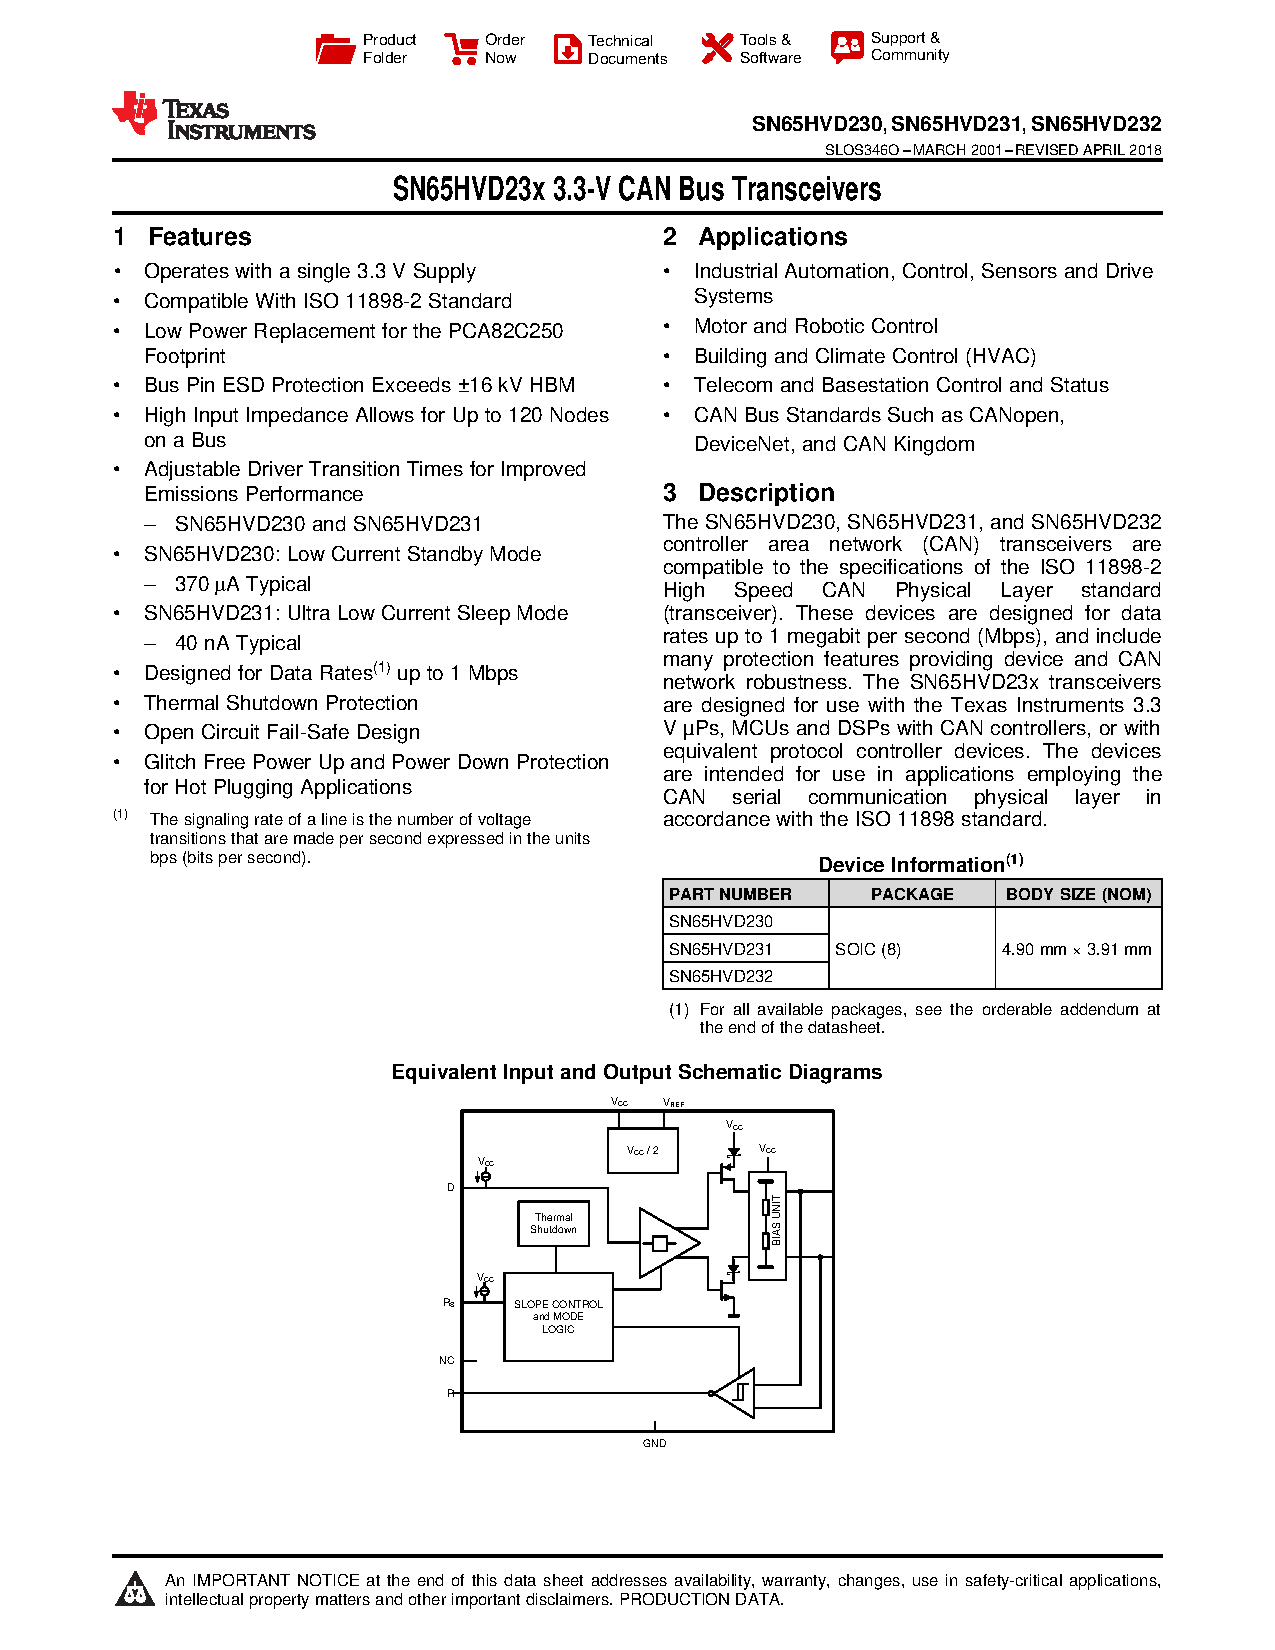
\includegraphics[page=1, width=0.95\textwidth]{DATASHEET/sn65hvd230.pdf}

	\vspace{4mm}
	\includegraphics[page=40, width=0.95\textwidth]{DATASHEET/sn65hvd230.pdf}
\end{center}

\newpage
\cleardoublepage % Limpia cualquier residuo de contadores anteriores
\refstepcounter{section}
\def\thesection{D} % <--- Fuerza a que el valor de la referencia sea solo "D"
\label{anexo:esp32}
\begin{center}
	\bfseries Apéndice D \\
	\normalfont\bfseries\itshape Hoja de Datos Técnicos del Módulo ESP32-S3-WROOM-1-N16R8
\end{center}
\addcontentsline{toc}{section}{Apéndice D: Hoja de Datos Técnicos del Módulo ESP32-S3-WROOM-1-N16R8}

\vspace{4mm}

Módulo Espressif ESP32-S3-WROOM-1-N16R8 (16~MB flash, 8~MB PSRAM octal), con controlador TWAI.

\begin{center}
	\includegraphics[page=2, width=0.91\textwidth]{DATASHEET/ESP32-S3.pdf}

	\vspace{4mm}
	\includegraphics[page=15, width=0.95\textwidth]{DATASHEET/ESP32-S3.pdf}

	
\end{center}

\newpage
\cleardoublepage % Limpia cualquier residuo de contadores anteriores
\refstepcounter{section}
\def\thesection{E} % <--- Fuerza a que el valor de la referencia sea solo "E"
\label{anexo:ssd1306}
\begin{center}
	\bfseries Apéndice E \\
	\normalfont\bfseries\itshape Hoja de Datos Técnicos del Controlador de Pantalla OLED SSD1306
\end{center}
\addcontentsline{toc}{section}{Apéndice E: Hoja de Datos Técnicos del Controlador de Pantalla OLED SSD1306}

\vspace{4mm}

Módulo de pantalla OLED I2C de 0,96", $128\times64$ píxeles, basado en el controlador SSD1306 \citep{ssd1306_datasheet}, con dirección I2C configurable entre \texttt{0x3C} y \texttt{0x3D}. Se reproducen las páginas de especificaciones básicas y el plano de dimensiones mecánicas del módulo.

\begin{center}
	\includegraphics[page=5, width=0.885\textwidth]{DATASHEET/OLED.pdf}

	\vspace{4mm}
	\includegraphics[page=6, width=0.95\textwidth]{DATASHEET/OLED.pdf}
\end{center}

\newpage
\cleardoublepage % Limpia cualquier residuo de contadores anteriores
\refstepcounter{section}
\def\thesection{F} % <--- Fuerza a que el valor de la referencia sea solo "F"
\label{anexo:fusible_ptc}
\begin{center}
	\bfseries Apéndice F \\
	\normalfont\bfseries\itshape Hoja de Datos Técnicos del Fusible PTC Reseteable, Serie BSMD1812
\end{center}
\addcontentsline{toc}{section}{Apéndice F: Hoja de Datos Técnicos del Fusible PTC Reseteable, Serie BSMD1812}

\vspace{4mm}

Fusible autorrecuperable PPTC de la serie BSMD1812 (encapsulado SMD 1812), con corriente de mantenimiento ($I_{hold}$) de 1{,}5~A y de disparo ($I_{trip}$) de 3{,}0~A \citep{bourns_bsmd1812}, primera línea de protección contra sobrecorriente en la línea de 12~V del conector OBD-II.

\begin{center}
	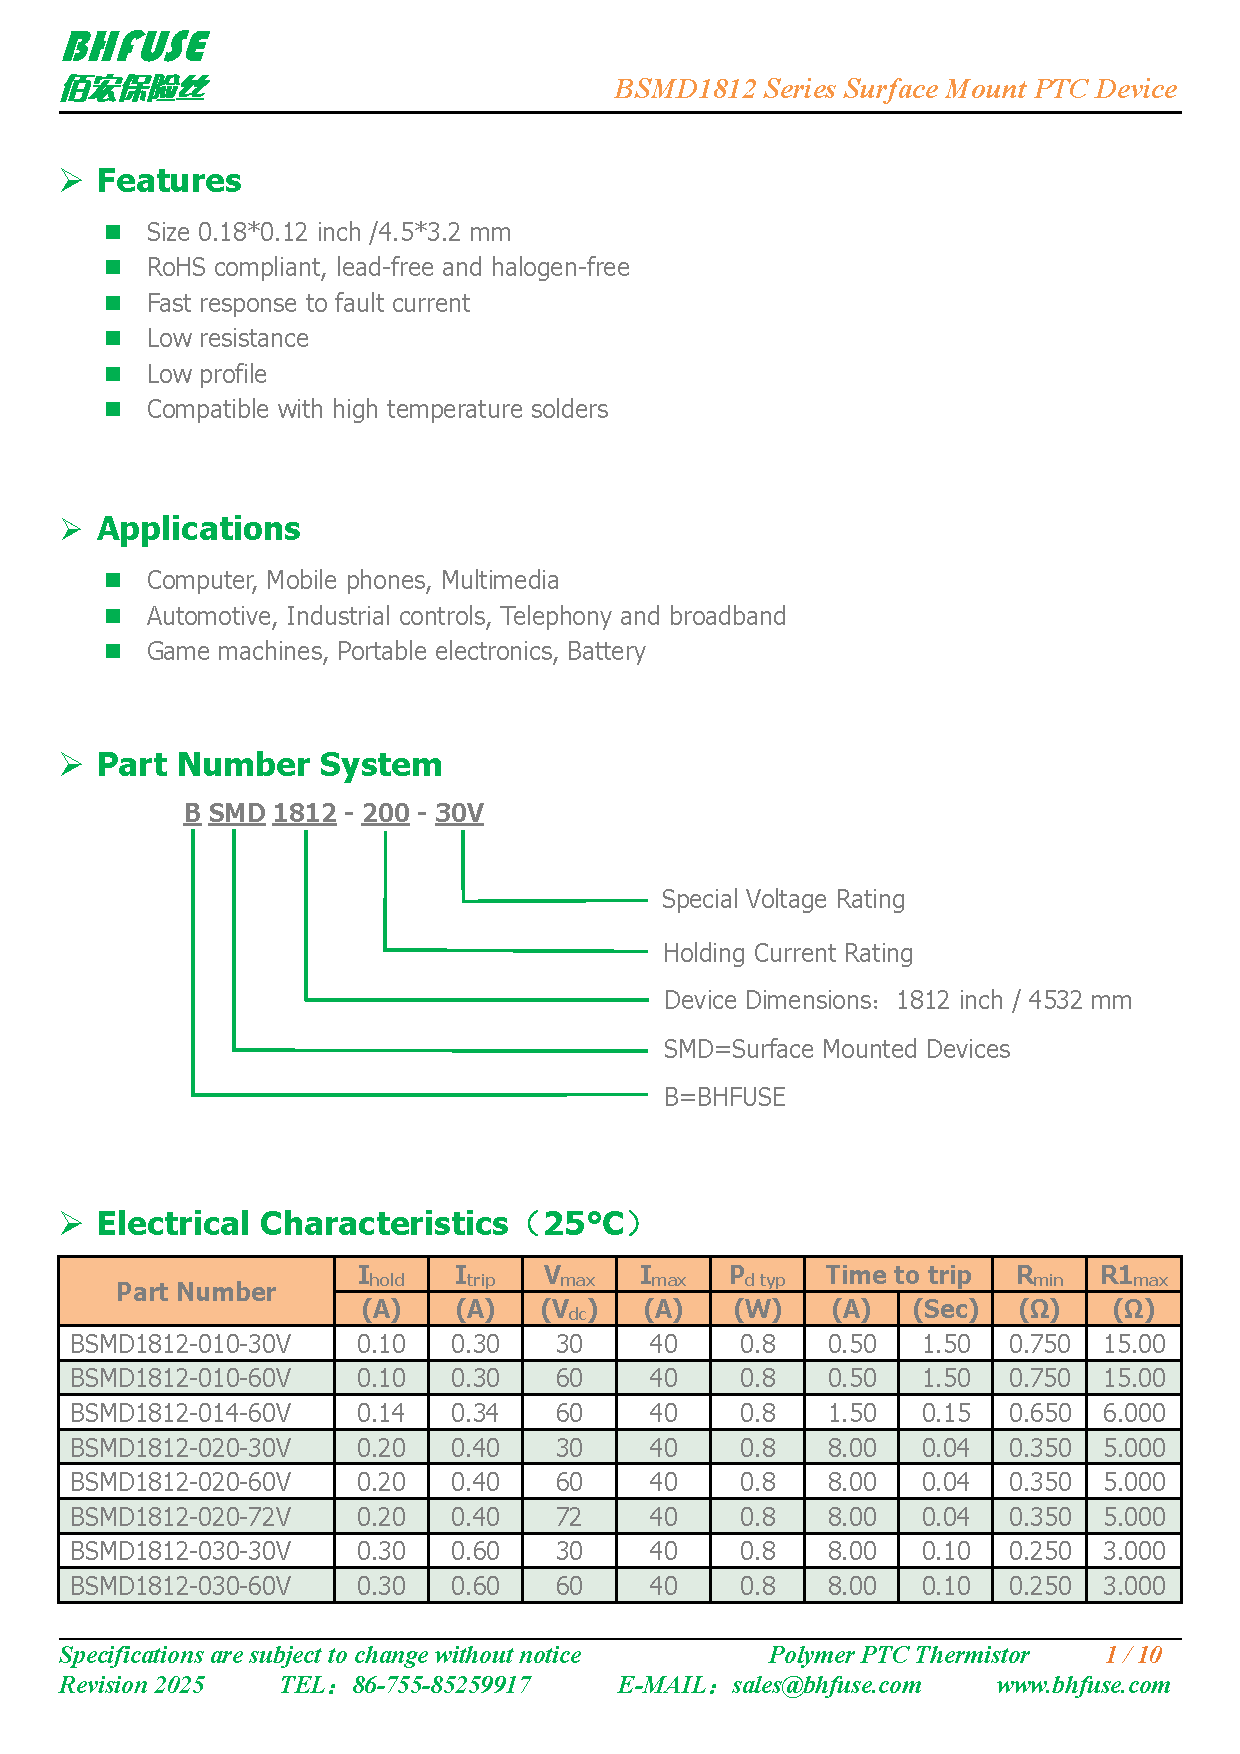
\includegraphics[page=1, width=0.85\textwidth]{DATASHEET/FUSE.pdf}
\end{center}

\newpage
\cleardoublepage
\refstepcounter{section}
\def\thesection{G}
\label{anexo:ss36}
\begin{center}
	\bfseries Apéndice G \\
	\normalfont\bfseries\itshape Diodo Schottky SS34 — Especificaciones Técnicas
\end{center}
\addcontentsline{toc}{section}{Apéndice G: Diodo Schottky SS34}

\vspace{4mm}

Diodo Schottky SS34 (familia SS32 a SS3200, MDD/China Base Electronics), encapsulado DO-214AC (SMA), con tensión inversa repetitiva máxima ($V_{RRM}$) de 40~V y corriente media rectificada ($I_O$) de 3~A \citep{onsemi_ss36}, usado como protección de polaridad inversa en la línea de 12~V del OBD-II. La fila correspondiente a SS34 es la aplicable a este proyecto.

\begin{center}
	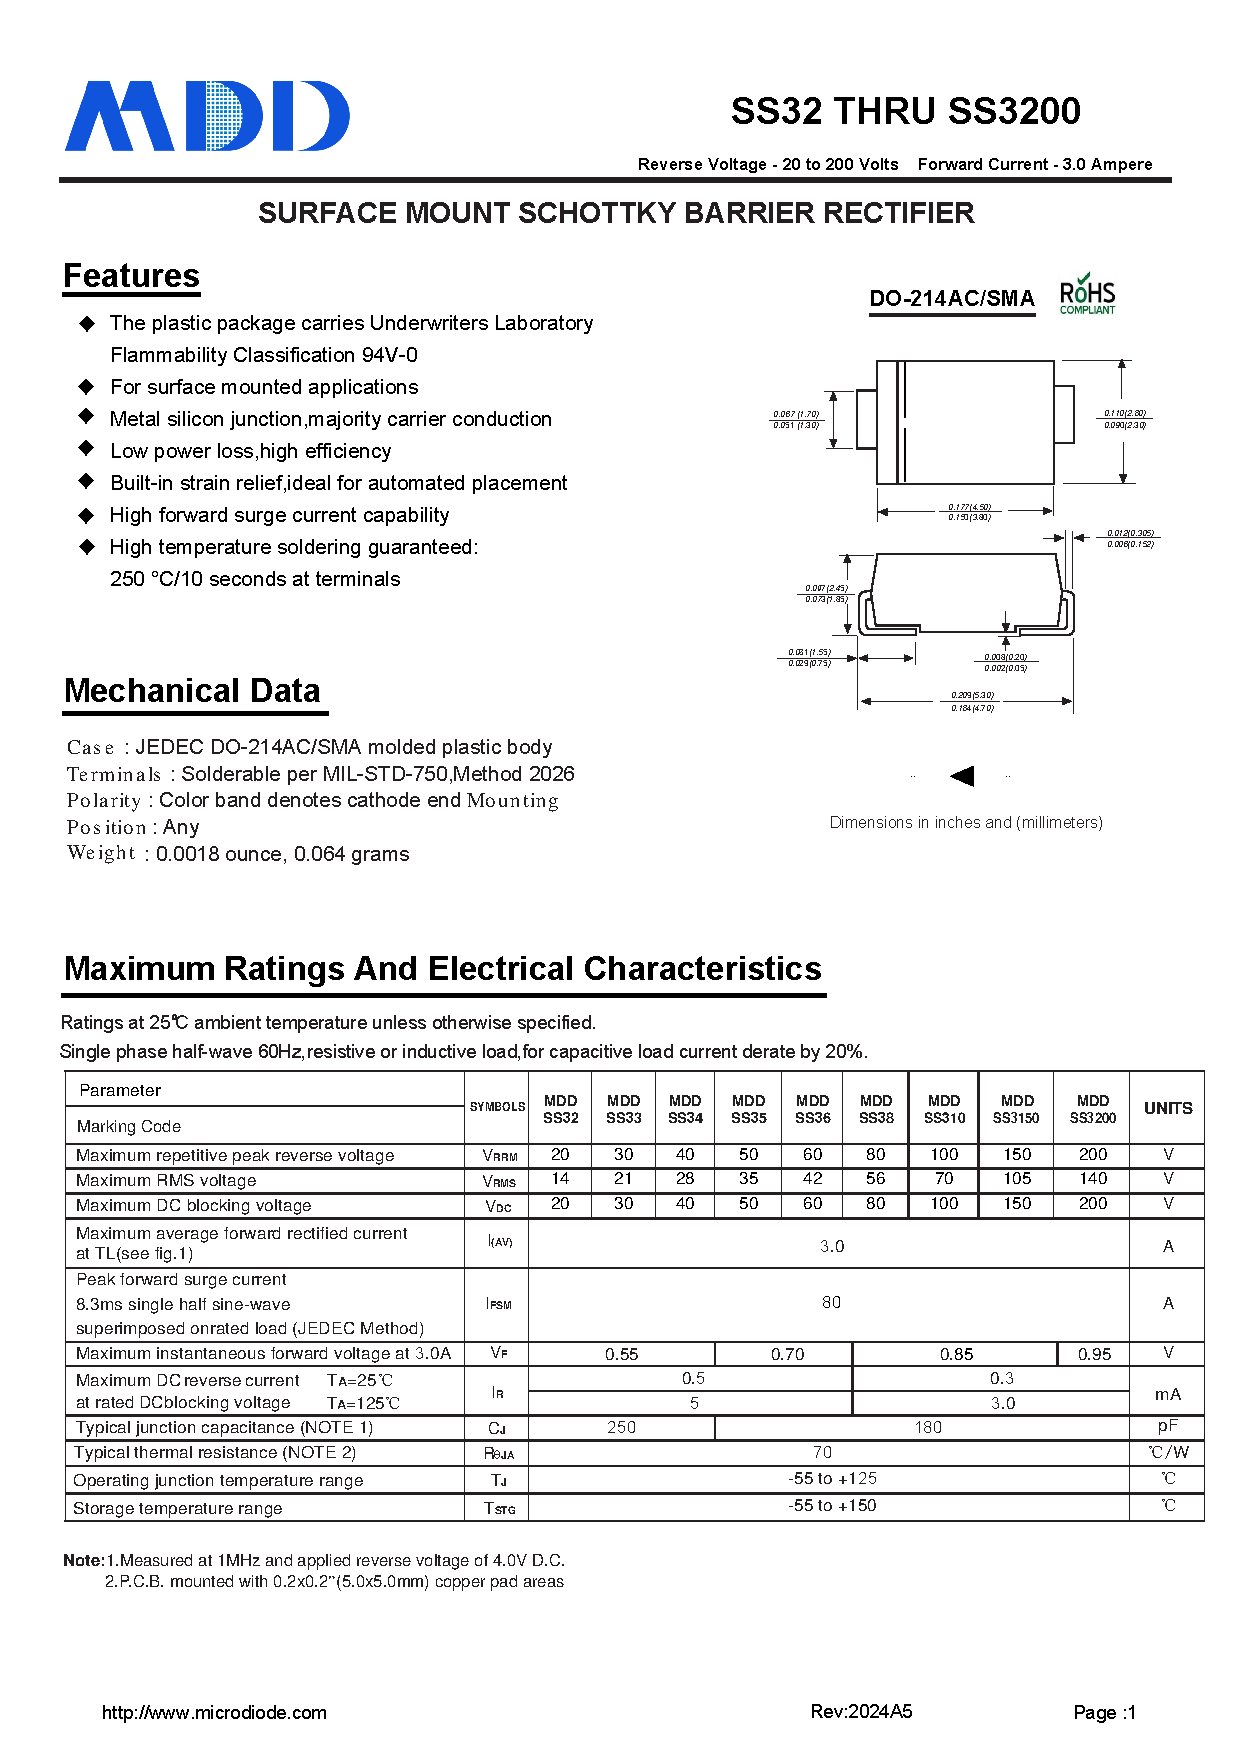
\includegraphics[page=1, width=0.85\textwidth]{DATASHEET/DIODE SS34.pdf}
\end{center}

\newpage
\cleardoublepage
\refstepcounter{section}
\def\thesection{H}
\label{apendiceG}
\begin{center}
	\bfseries Apéndice H \\
	\normalfont\bfseries\itshape Hoja de Datos Técnicos del Diodo Supresor de Tensión Transitoria (TVS) SMAJ18A
\end{center}
\addcontentsline{toc}{section}{Apéndice H: Hoja de Datos Técnicos del Diodo Supresor de Tensión Transitoria (TVS) SMAJ18A}

\vspace{4mm}

Diodo TVS Littelfuse serie SMAJ, modelo SMAJ18A (DO-214AC/SMA, 400~W pico), con tensión de trabajo (\textit{stand-off}) de 18~V y tensión de sujeción máxima de 29{,}2~V a 13{,}7~A \citep{vishay_smaj28a}, usado como protección contra transitorios de \textit{load dump} y ESD en la línea de 12~V.

\begin{center}
	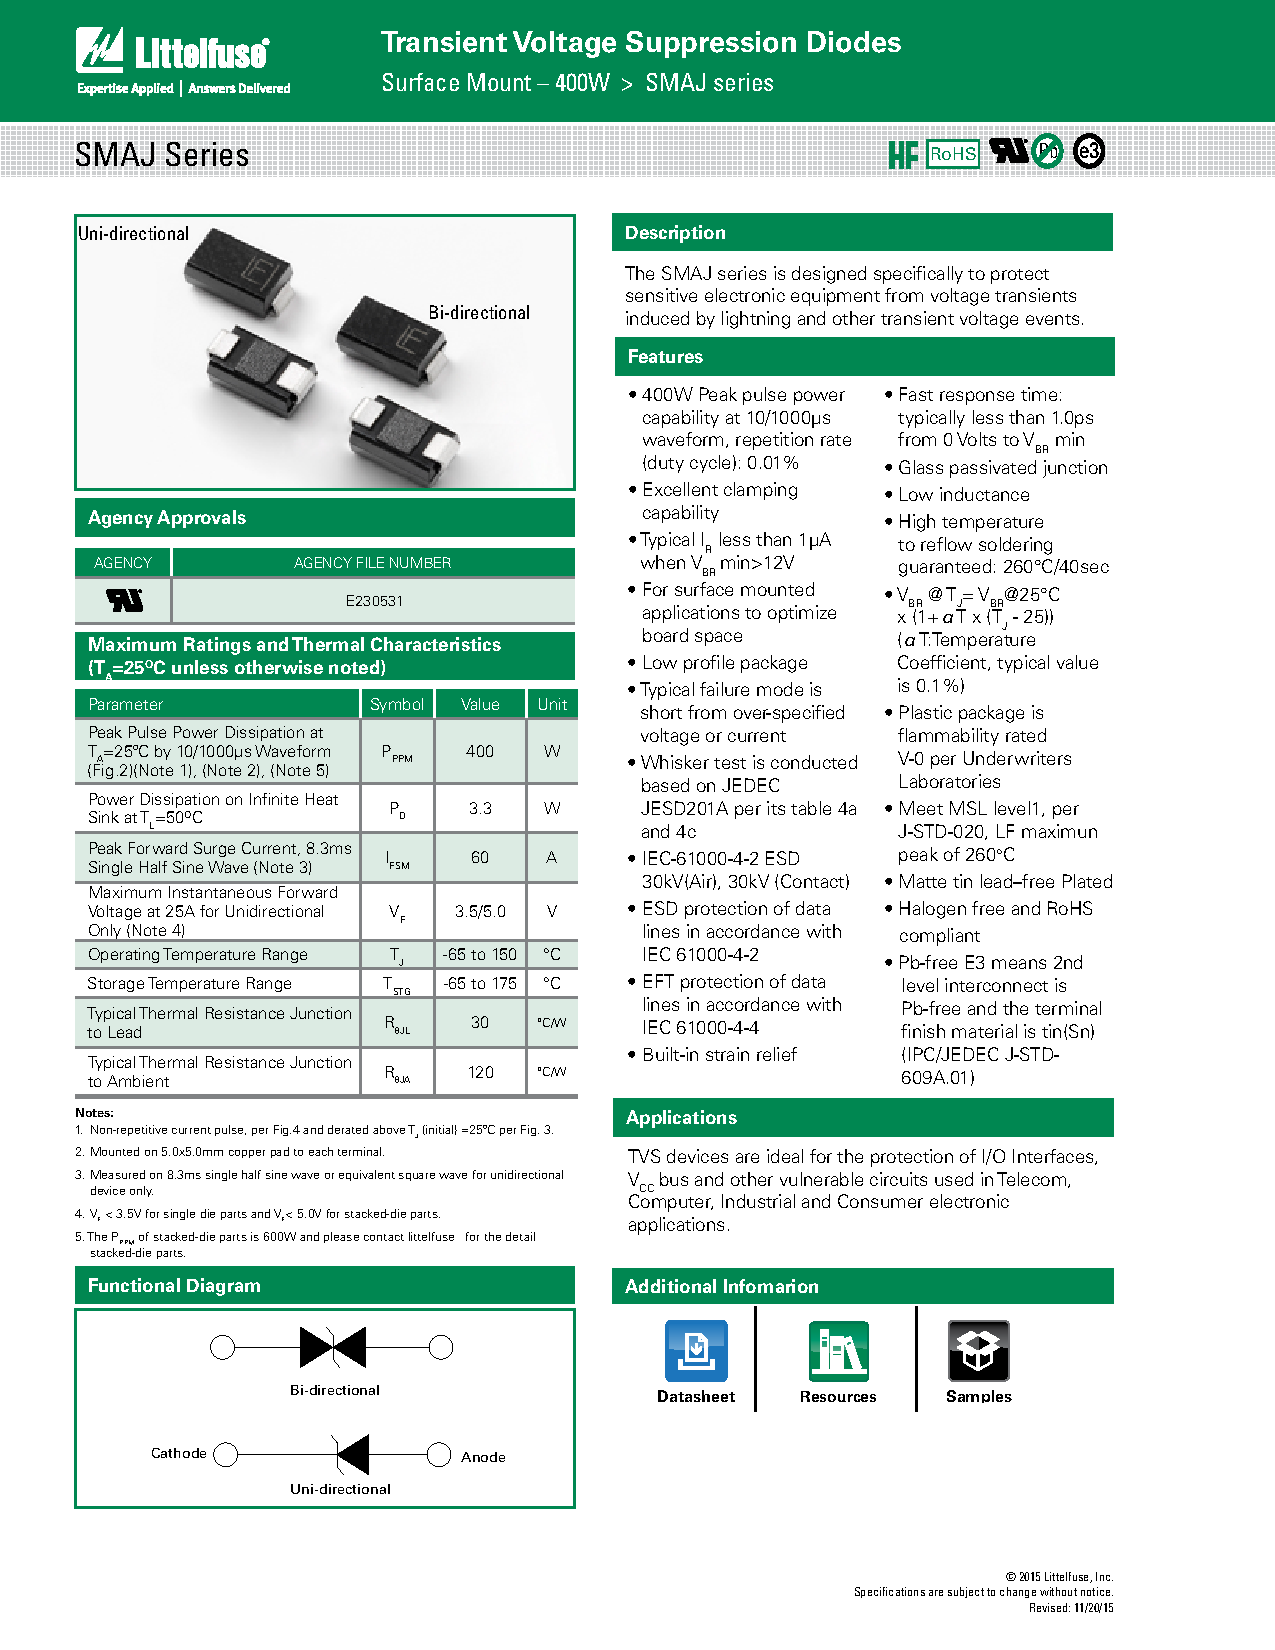
\includegraphics[page=1, width=0.85\textwidth]{DATASHEET/SMAJ18A.pdf}
\end{center}

\newpage
\cleardoublepage
\refstepcounter{section}
\def\thesection{I}
\label{anexo:tps54302}
\begin{center}
	\bfseries Apéndice I \\
	\normalfont\bfseries\itshape Hoja de Datos Técnicos del Convertidor Buck Síncrono TPS54302DDCR
\end{center}
\addcontentsline{toc}{section}{Apéndice I: Hoja de Datos Técnicos del Convertidor Buck Síncrono TPS54302DDCR}

\vspace{4mm}

Convertidor \textit{buck} síncrono TPS54302DDCR (Texas Instruments), primera etapa de la cadena de regulación de dos rieles (Capítulo~3): 12~V~$\rightarrow$~5~V, entrada de 4{,}5~V a 28~V, hasta 3~A continuos a 400~kHz, encapsulado SOT-23-6. Se reproducen las páginas de características y de dimensiones del encapsulado.

\begin{center}
	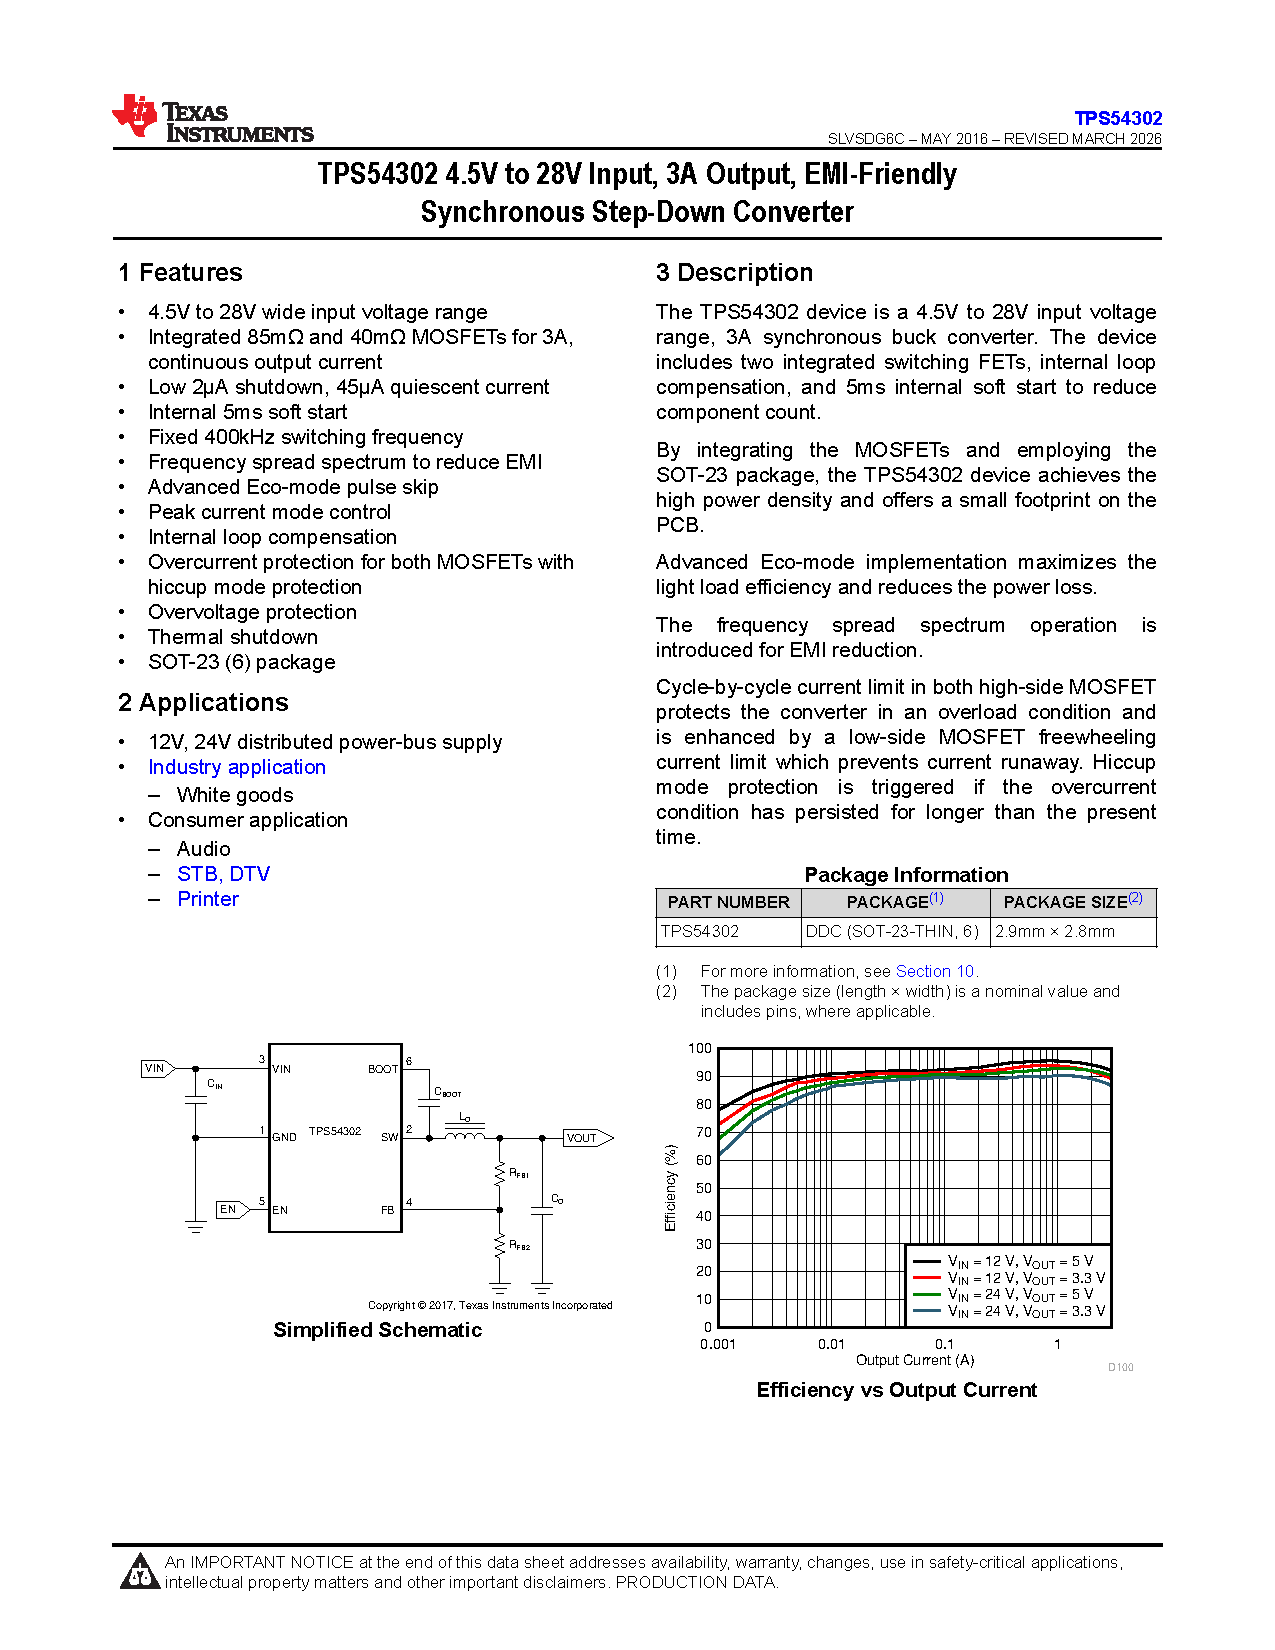
\includegraphics[page=1, width=0.85\textwidth]{DATASHEET/TPS54302.pdf}

	\vspace{4mm}
	\includegraphics[page=14, width=0.98\textwidth]{DATASHEET/TPS54302.pdf}
\end{center}

\newpage
\cleardoublepage
\refstepcounter{section}
\def\thesection{J}
\label{anexo:ams1117}
\begin{center}
	\bfseries Apéndice J \\
	\normalfont\bfseries\itshape Hoja de Datos Técnicos del Regulador Lineal AMS1117-3.3
\end{center}
\addcontentsline{toc}{section}{Apéndice J: Hoja de Datos Técnicos del Regulador Lineal AMS1117-3.3}

\vspace{4mm}

LDO AMS1117-3.3, alimenta el riel~1 permanentemente activo (ESP32-S3-WROOM-1-N16R8 y SN65HVD230) a partir de los 5~V del TPS54302DDCR (Apéndice~I), con capacidad de hasta 1~A continuo.

\begin{center}
	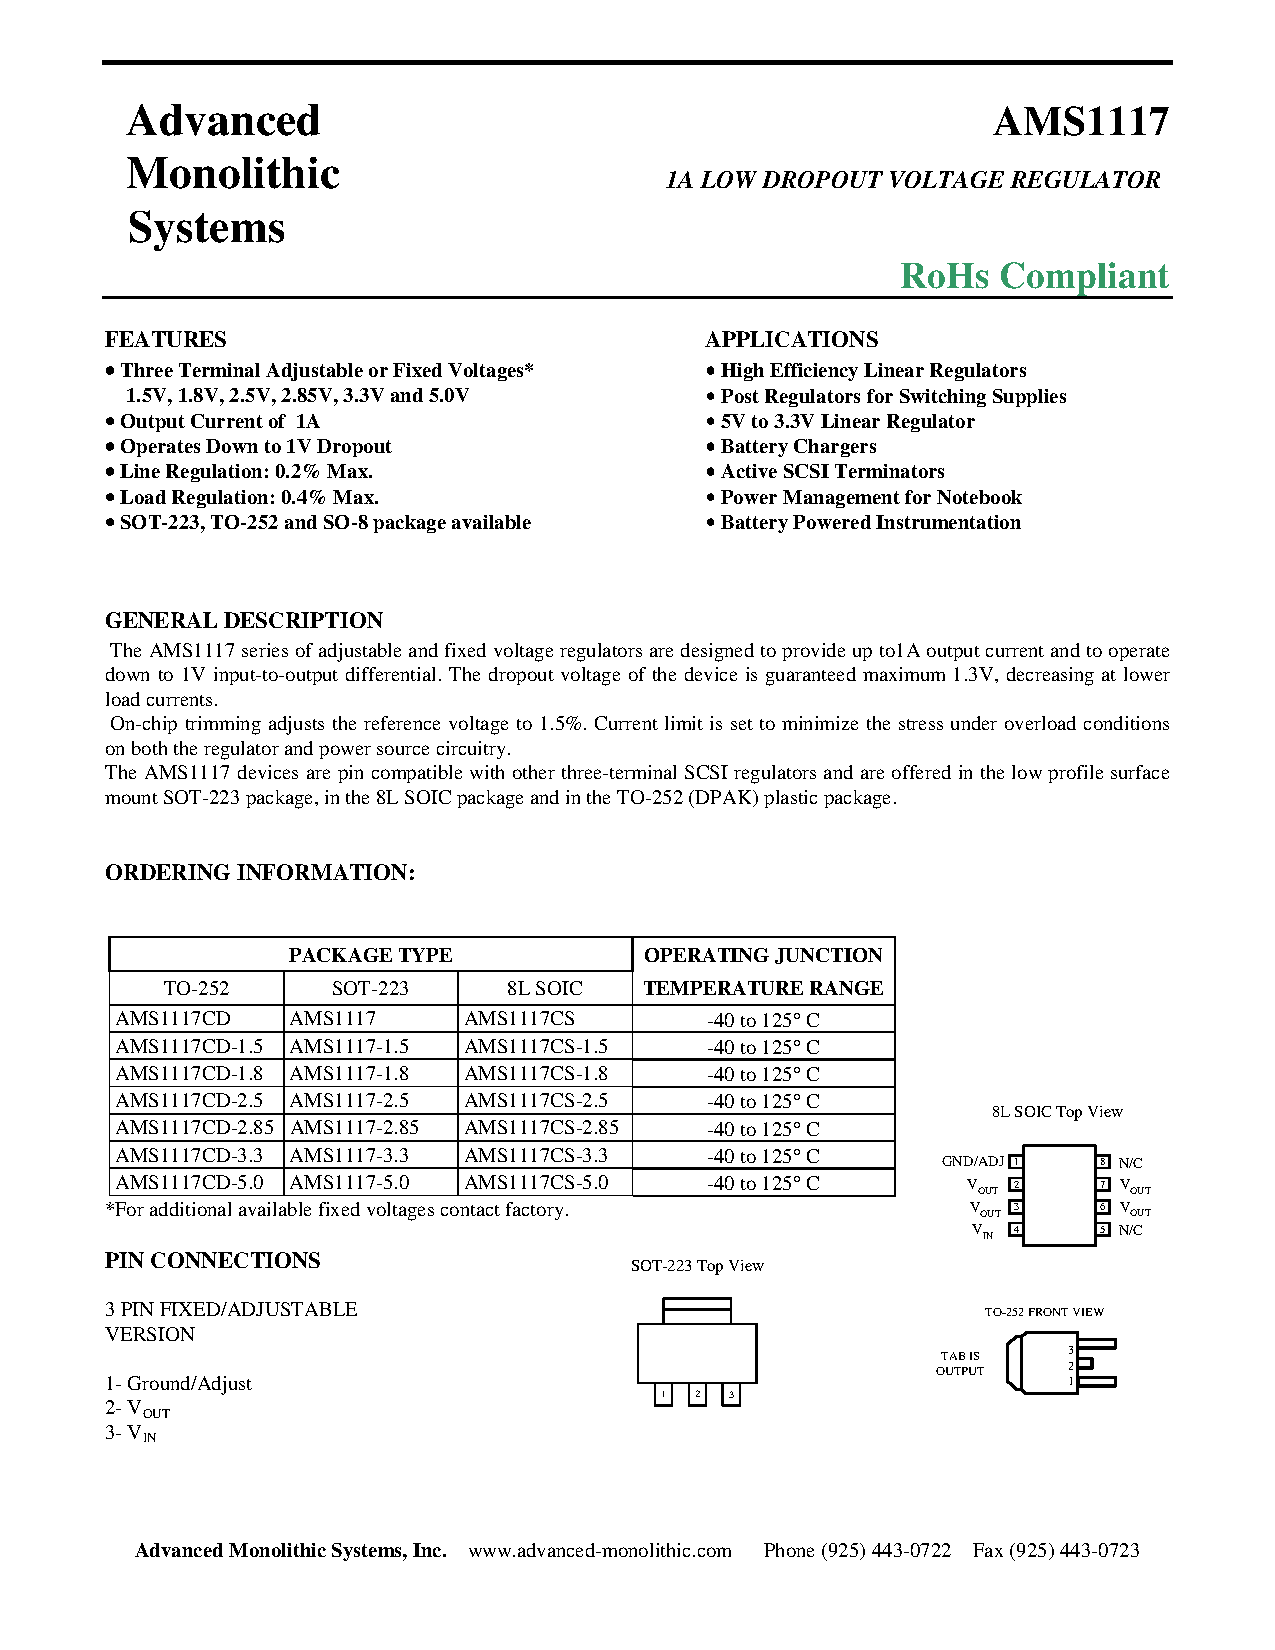
\includegraphics[page=1, width=0.95\textwidth]{DATASHEET/AMS1117.pdf}
\end{center}

\newpage
\cleardoublepage
\refstepcounter{section}
\def\thesection{K}
\label{anexo:ap2112k}
\begin{center}
	\bfseries Apéndice K \\
	\normalfont\bfseries\itshape Hoja de Datos Técnicos del Regulador Lineal AP2112K-3.3TRG1
\end{center}
\addcontentsline{toc}{section}{Apéndice K: Hoja de Datos Técnicos del Regulador Lineal AP2112K-3.3TRG1}

\vspace{4mm}

LDO AP2112K-3.3TRG1 (Diodes Incorporated), alimenta el riel~2 conmutado (OLED, microSD) vía el interruptor de carga TPS22918 (Apéndice~L), con capacidad de hasta 600~mA y bajo nivel de ruido.

\begin{center}
	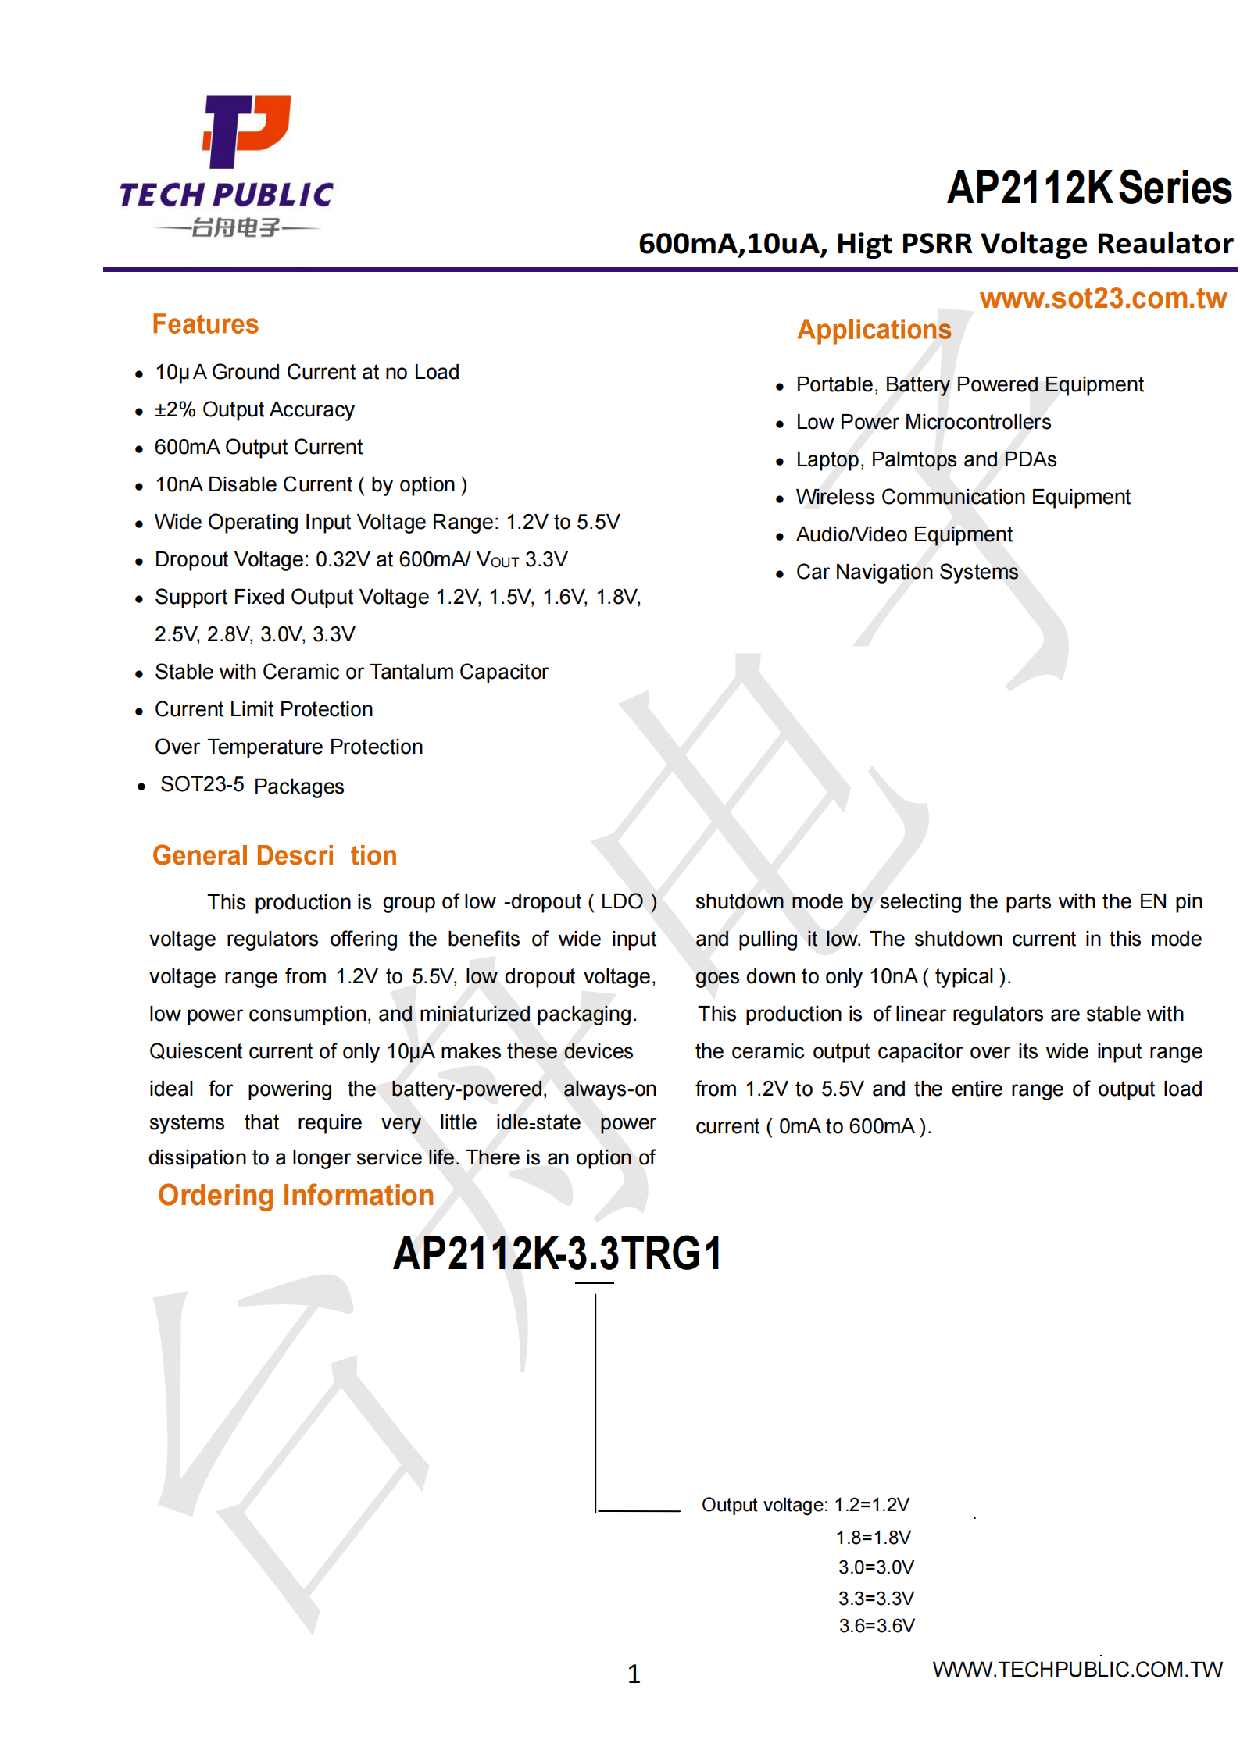
\includegraphics[page=1, width=0.85\textwidth]{DATASHEET/AP2112K.pdf}
\end{center}

\newpage
\cleardoublepage
\refstepcounter{section}
\def\thesection{L}
\label{anexo:tps22918}
\begin{center}
	\bfseries Apéndice L \\
	\normalfont\bfseries\itshape Hoja de Datos Técnicos del Interruptor de Carga TPS22918
\end{center}
\addcontentsline{toc}{section}{Apéndice L: Hoja de Datos Técnicos del Interruptor de Carga TPS22918}

\vspace{4mm}

Interruptor de carga (\textit{load switch}) TPS22918 (Texas Instruments), conecta/desconecta el riel~2 de 3{,}3~V (OLED, microSD) bajo control de un GPIO del ESP32-S3, implementando el modo de bajo consumo del Capítulo~3. $R_{ON}\approx 52\,\text{m}\Omega$, control configurable del tiempo de subida.

\begin{center}
	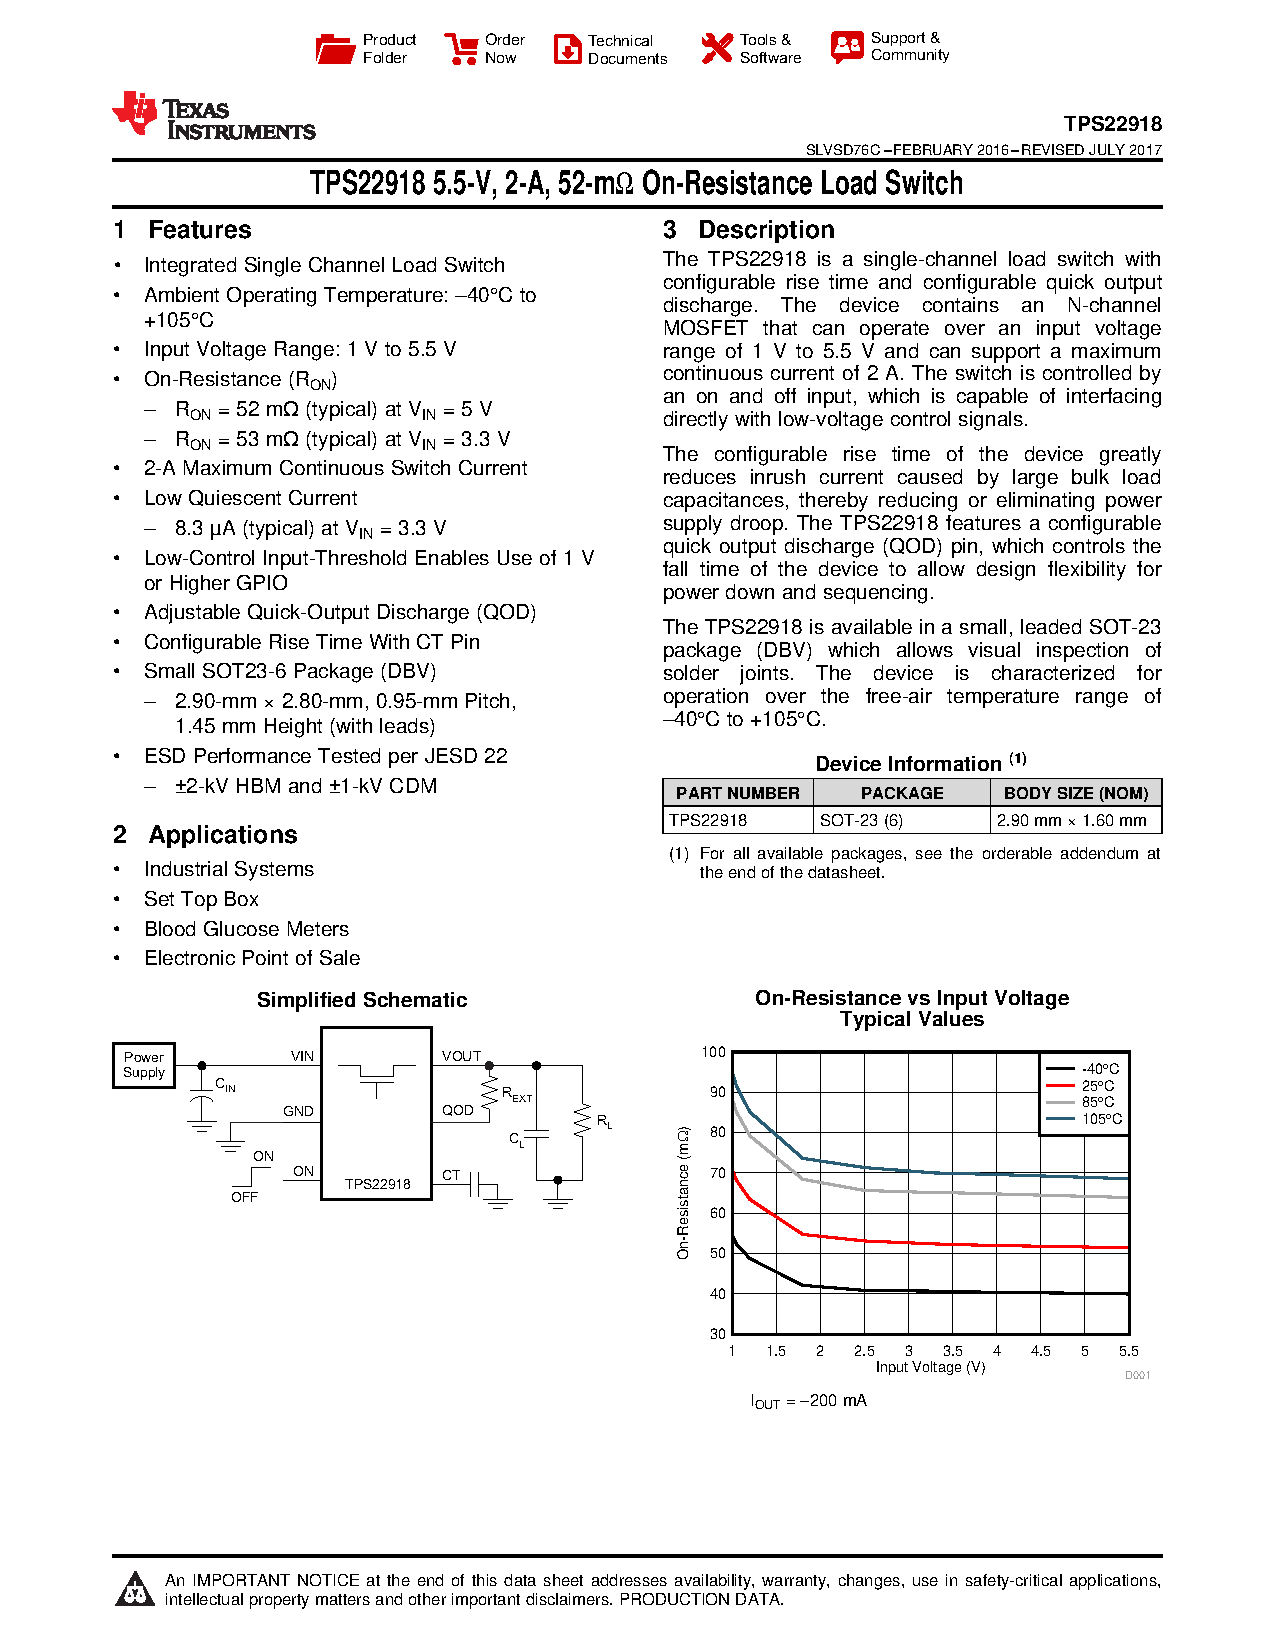
\includegraphics[page=1, width=0.95\textwidth]{DATASHEET/TPS22918.pdf}

	\vspace{4mm}
	\includegraphics[page=16, width=1\textwidth]{DATASHEET/TPS22918.pdf}

	\vspace{4mm}
	\includegraphics[page=18, width=1\textwidth]{DATASHEET/TPS22918.pdf}
\end{center}

\newpage
\cleardoublepage
\refstepcounter{section}
\def\thesection{M}
\label{anexo:esquematico_pcb}
\begin{center}
	\bfseries Apéndice M \\
	\normalfont\bfseries\itshape Esquemático Eléctrico Completo y Diseño de la PCB
\end{center}
\addcontentsline{toc}{section}{Apéndice M: Esquemático Eléctrico Completo y Diseño de la PCB}

\vspace{4mm}

Esquemático eléctrico completo del sistema (diseñado en Altium Designer), disposición física de la PCB (vista de capas y ruteado) y reporte de la pila de capas (\textit{board stack}), referenciados desde la Sección de diseño de hardware del Capítulo~3.

\begin{center}
	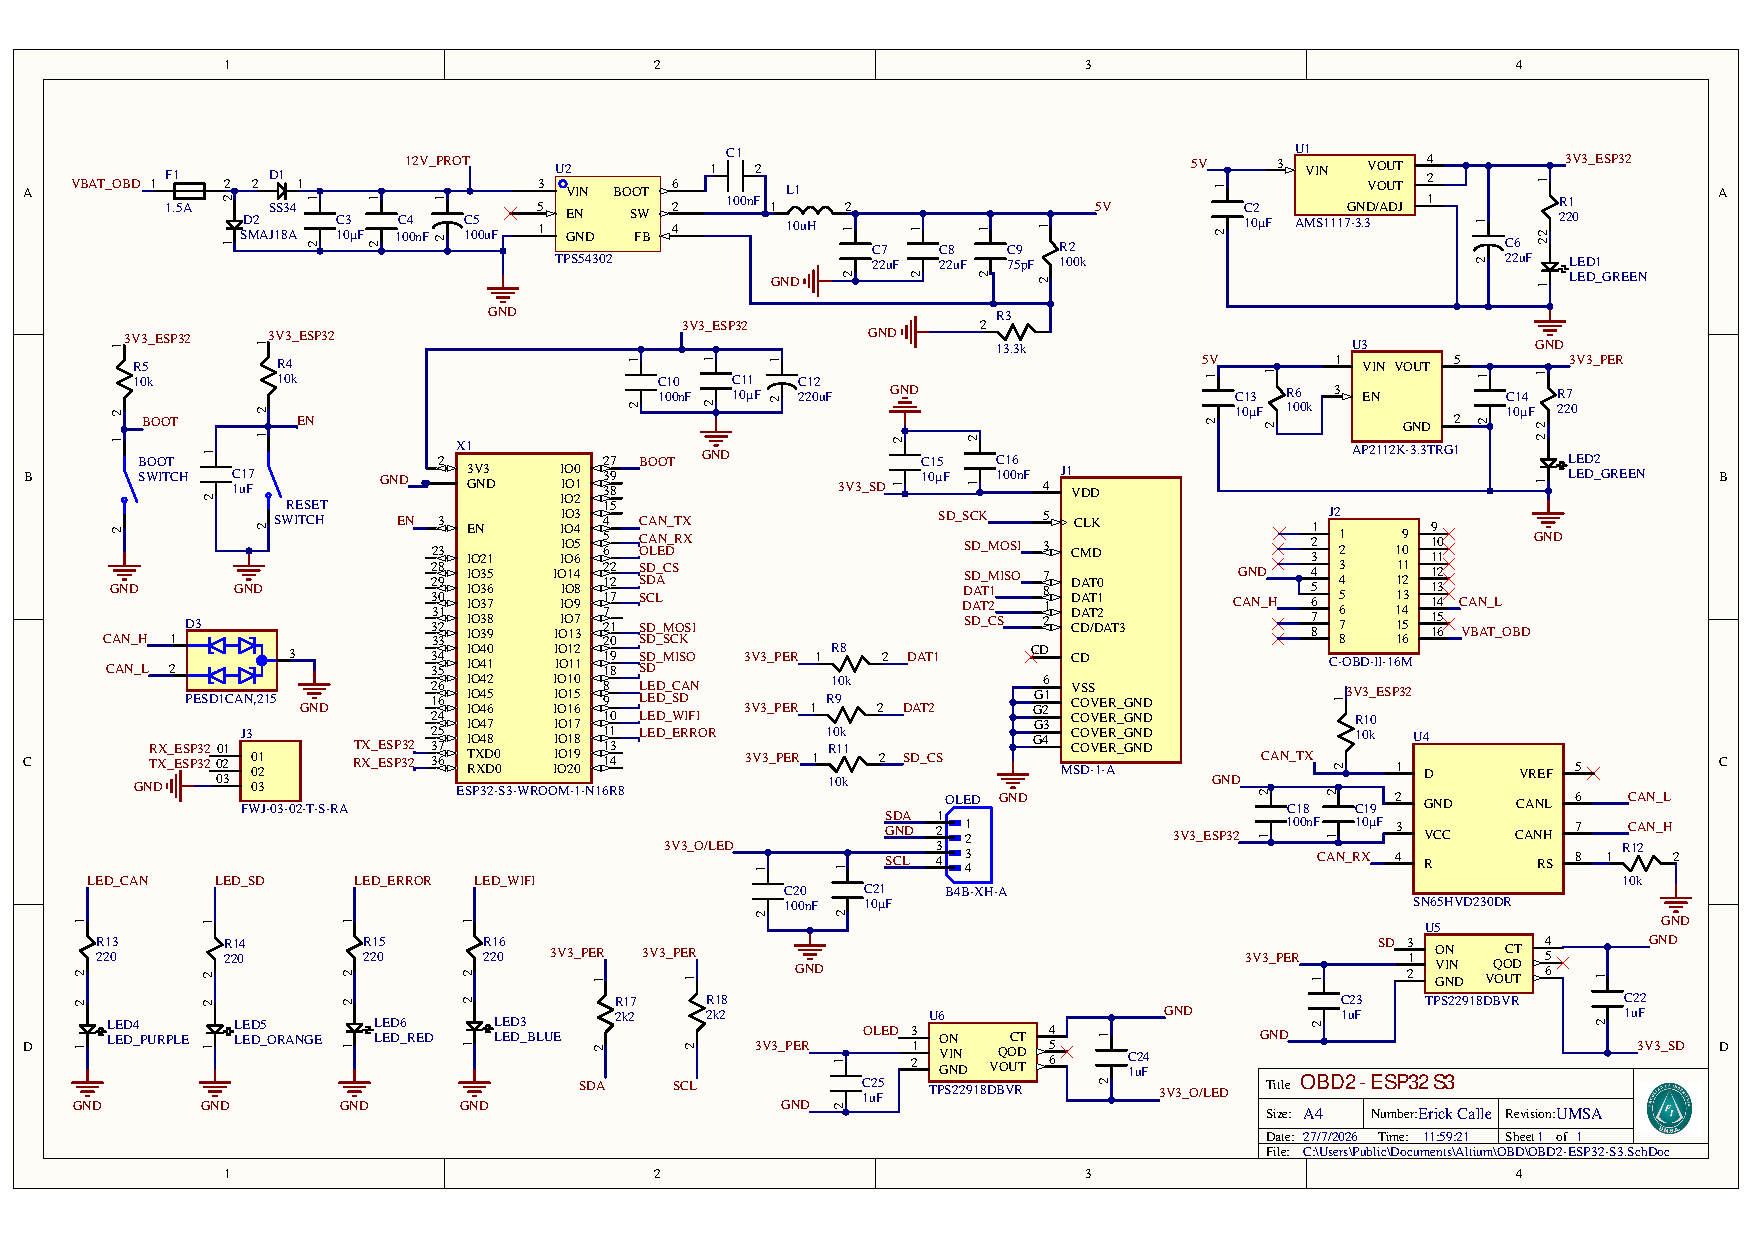
\includegraphics[page=1, width=\textwidth]{DATASHEET/OBD2.pdf}

	\vspace{4mm}
	\includegraphics[page=2, width=0.7\textwidth]{DATASHEET/OBD2.pdf}

\end{center}

\newpage
\cleardoublepage
\refstepcounter{section}
\def\thesection{N}
\label{anexo:bom_detalle}
\begin{center}
	\bfseries Apéndice N \\
	\normalfont\bfseries\itshape Lista de Materiales (BOM) — Detalle de Fabricación
\end{center}
\addcontentsline{toc}{section}{Apéndice N: Lista de Materiales (BOM) — Detalle de Fabricación}

\vspace{4mm}

A diferencia de la Tabla~\ref{bom} del Capítulo~3 —que agrupa los componentes por bloque funcional con fines explicativos—, este apéndice reproduce la lista de materiales tal como se exportó para la fabricación y el ensamblaje de la PCB.
\begin{center}
	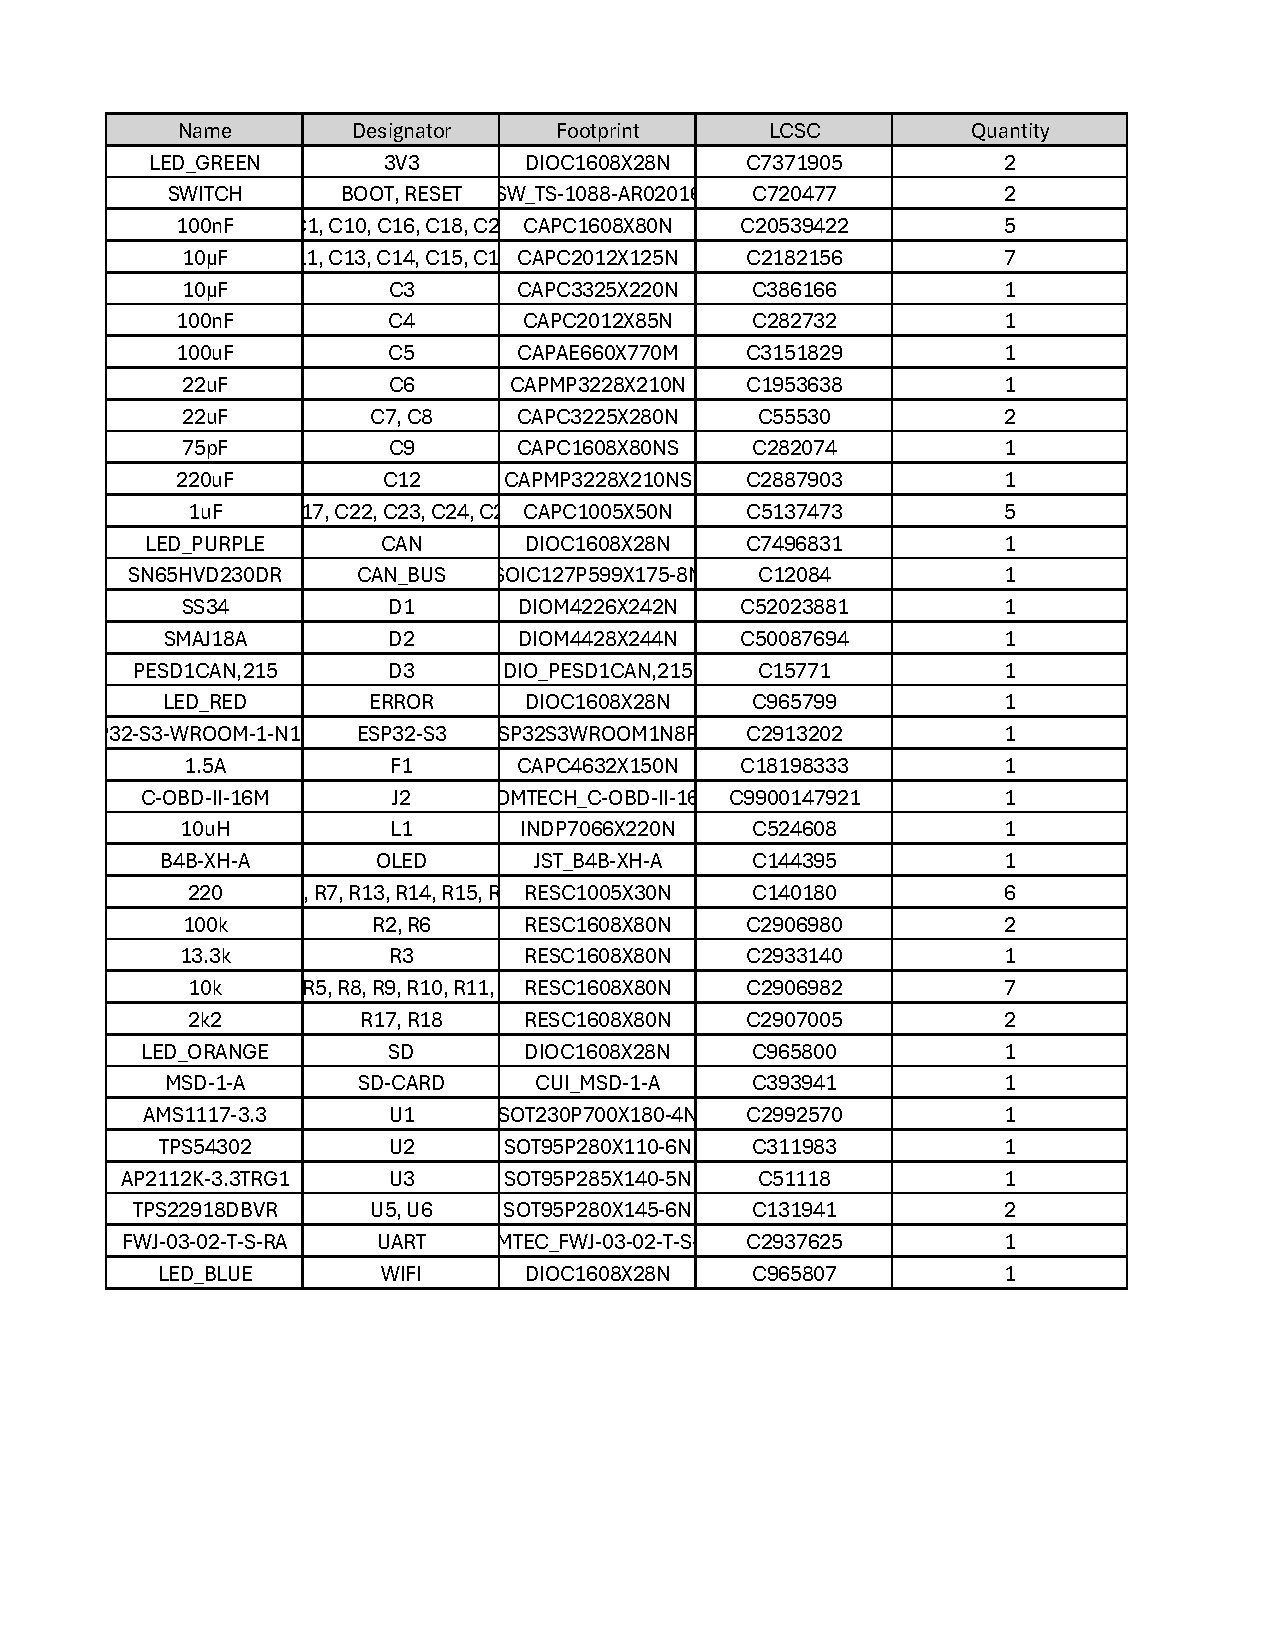
\includegraphics[page=1, width=0.92\textwidth]{DATASHEET/BOOM.pdf}
\end{center}

\newpage
\cleardoublepage
\refstepcounter{section}
\def\thesection{O}
\label{anexo:pids_vehiculos}
\begin{center}
	\bfseries Apéndice O \\
	\normalfont\bfseries\itshape PIDs OBD-II Soportados por los Vehículos de Prueba: Changan Honor y Nissan Vanette
\end{center}
\addcontentsline{toc}{section}{Apéndice O: PIDs OBD-II Soportados por los Vehículos de Prueba}

\vspace{4mm}

Listado completo y decodificado de los PIDs OBD-II (Modo~01) soportados por cada vehículo de validación, obtenido mediante el escaneo activo del Capítulo~3. Changan Honor: 34 PIDs, sin el PID~0x10 (MAF). Nissan Vanette: 33 PIDs, incluyendo el PID~0x10.

\begin{center}
	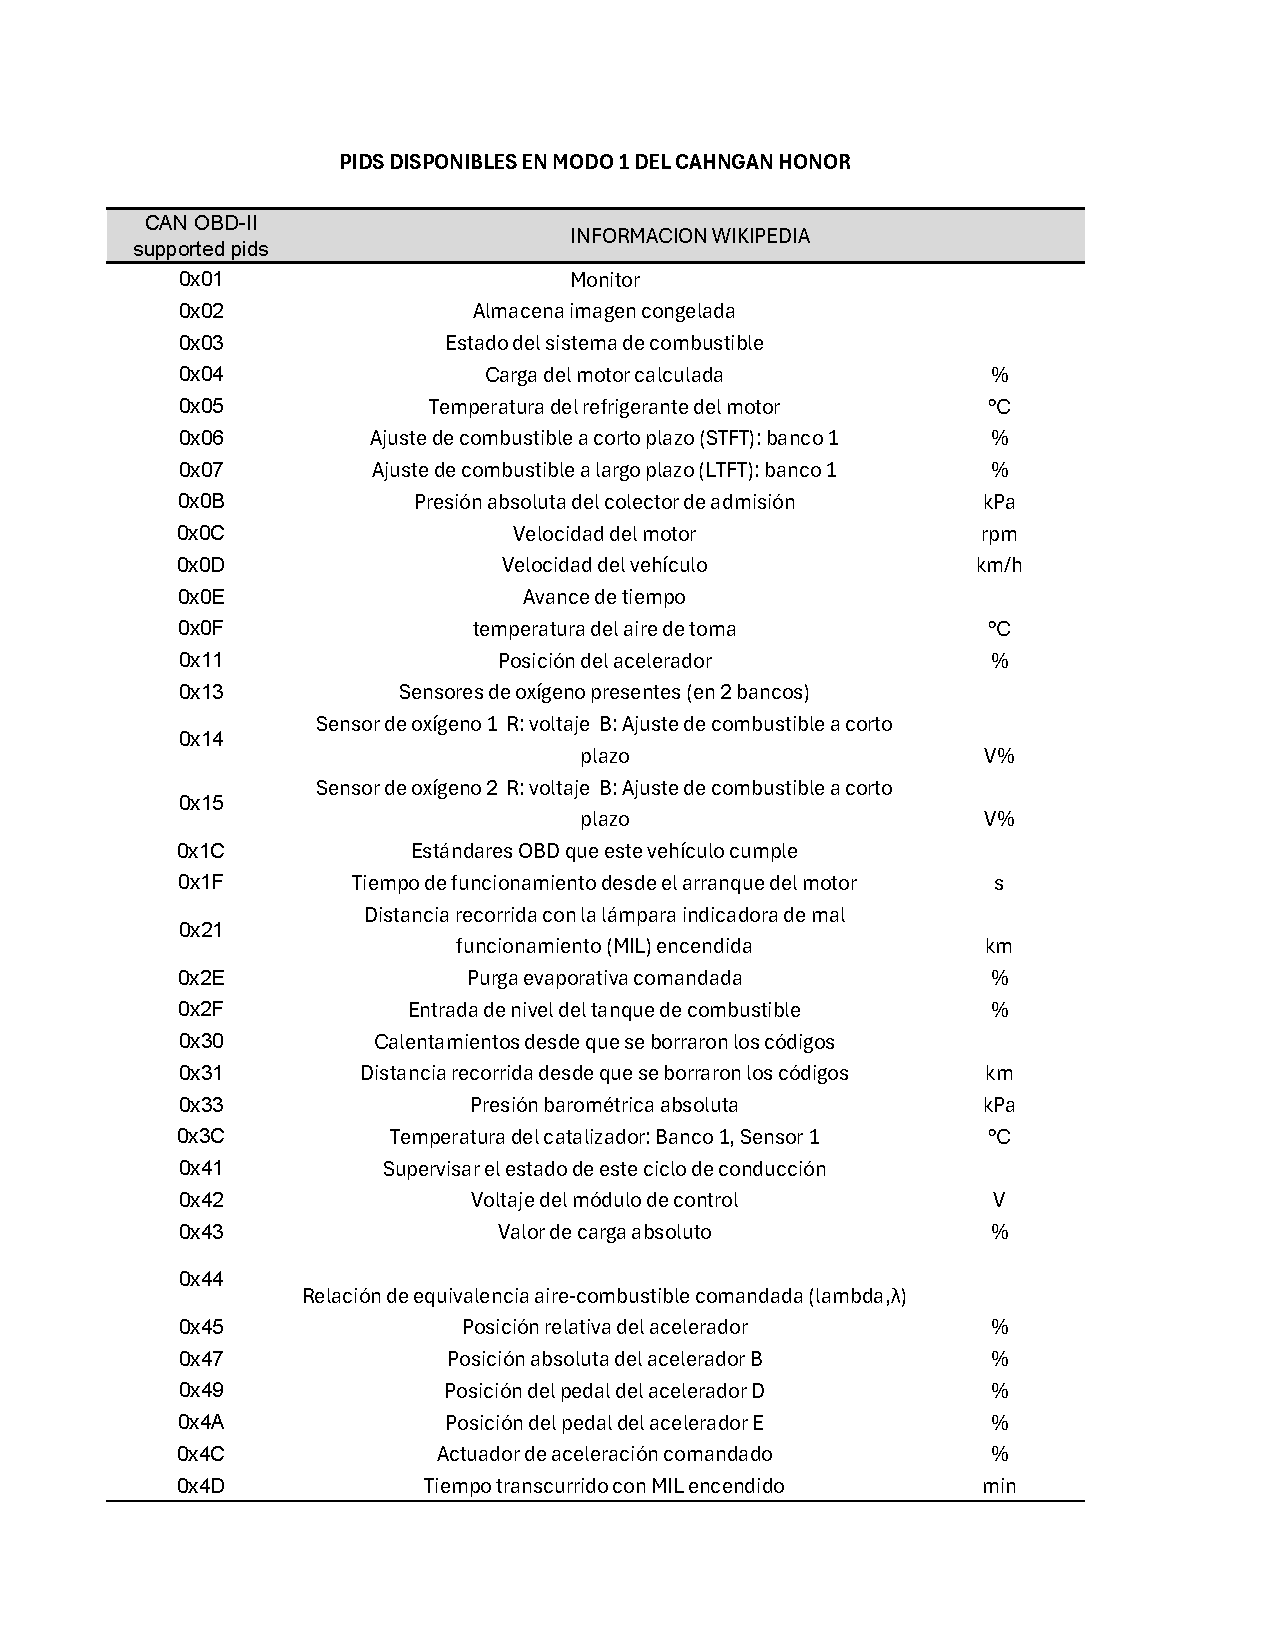
\includegraphics[page=1, width=0.94\textwidth]{DATASHEET/CHANGAN.pdf}

	\vspace{4mm}
	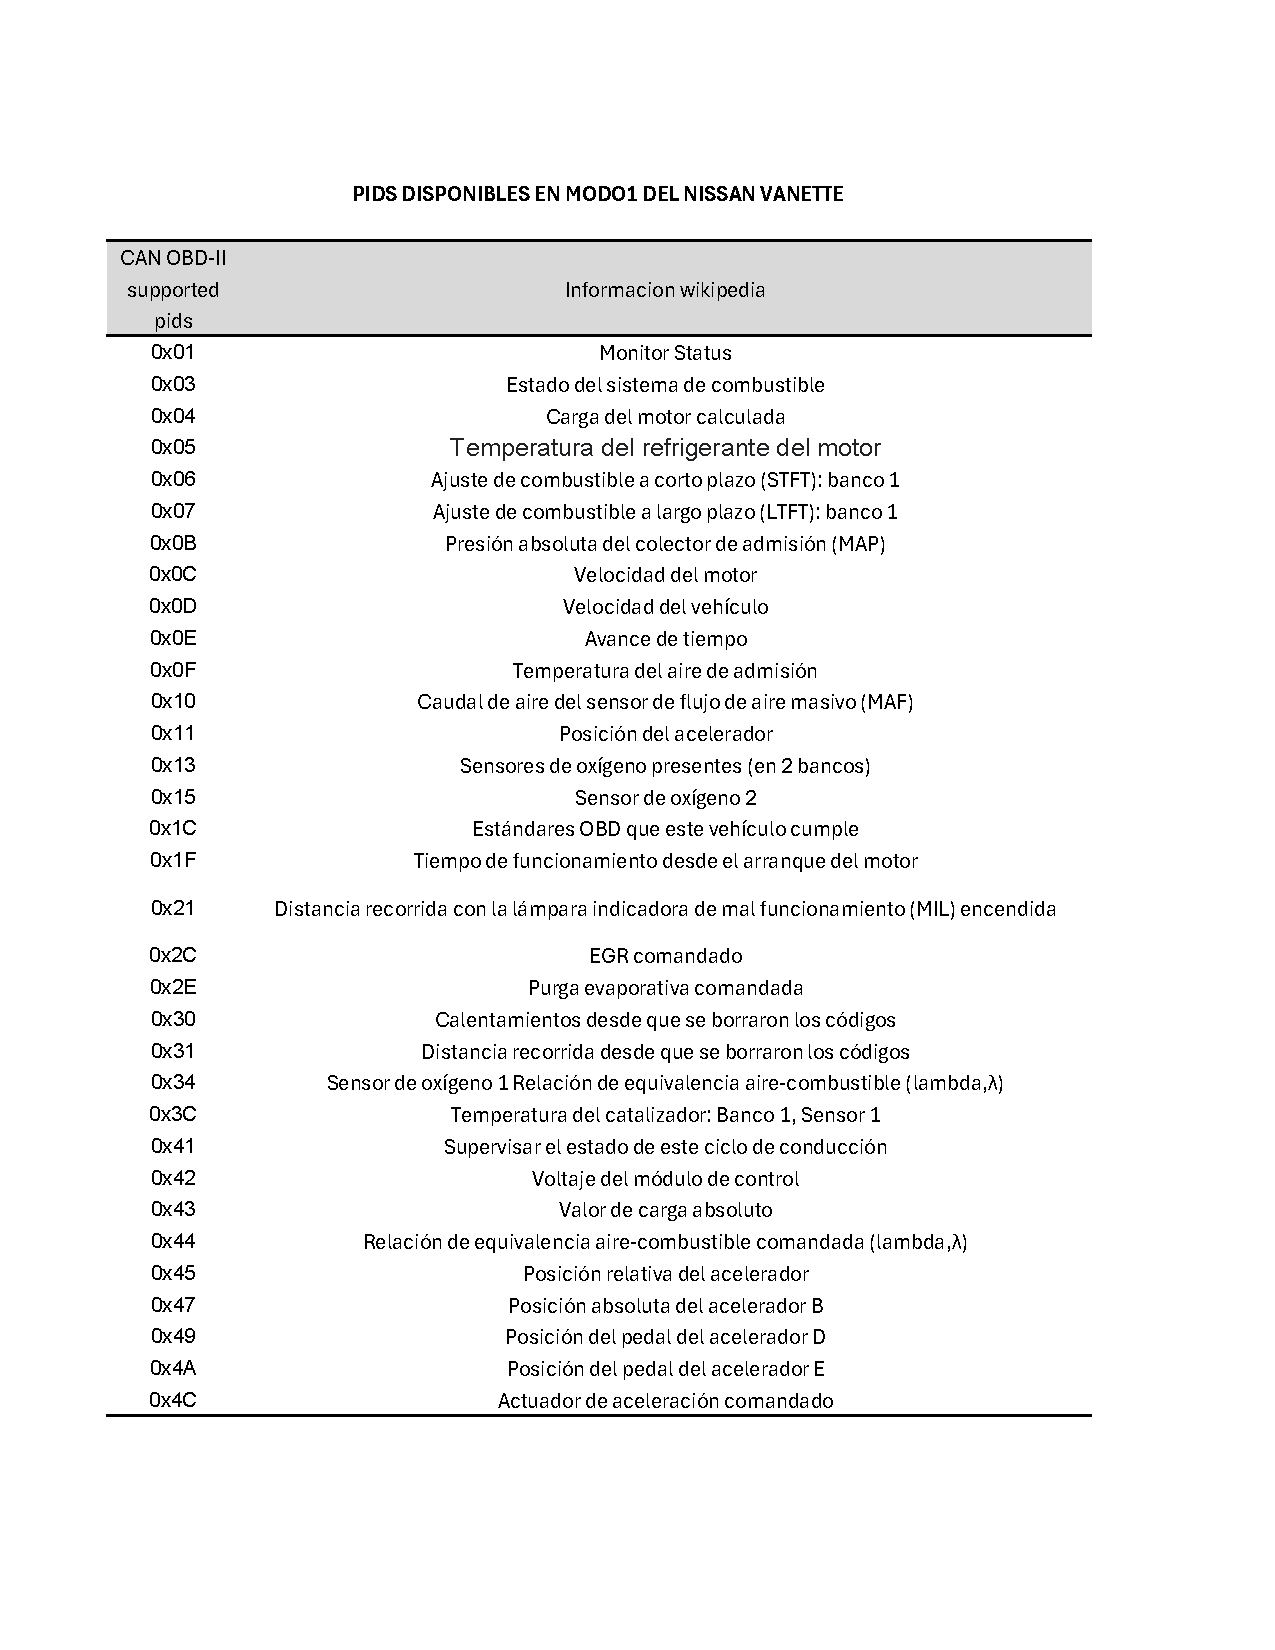
\includegraphics[page=1, width=1.1\textwidth]{DATASHEET/NISSAN.pdf}
\end{center}

\newpage
\cleardoublepage
\refstepcounter{section}
\def\thesection{P}
\label{anexo:mcp2515}
\begin{center}
	\bfseries Apéndice P \\
	\normalfont\bfseries\itshape Hoja de Datos Técnicos del Controlador CAN MCP2515 (Arquitectura Descartada)
\end{center}
\addcontentsline{toc}{section}{Apéndice P: Hoja de Datos Técnicos del Controlador CAN MCP2515 (Arquitectura Descartada)}

\vspace{4mm}

Controlador CAN independiente con interfaz SPI (Microchip), evaluado en la etapa inicial del proyecto y descartado en favor del periférico TWAI integrado en el ESP32-S3-WROOM-1-N16R8 (Apéndice~D). Se documenta únicamente como referencia del proceso de decisión de diseño, no como componente del sistema final.

\begin{center}
	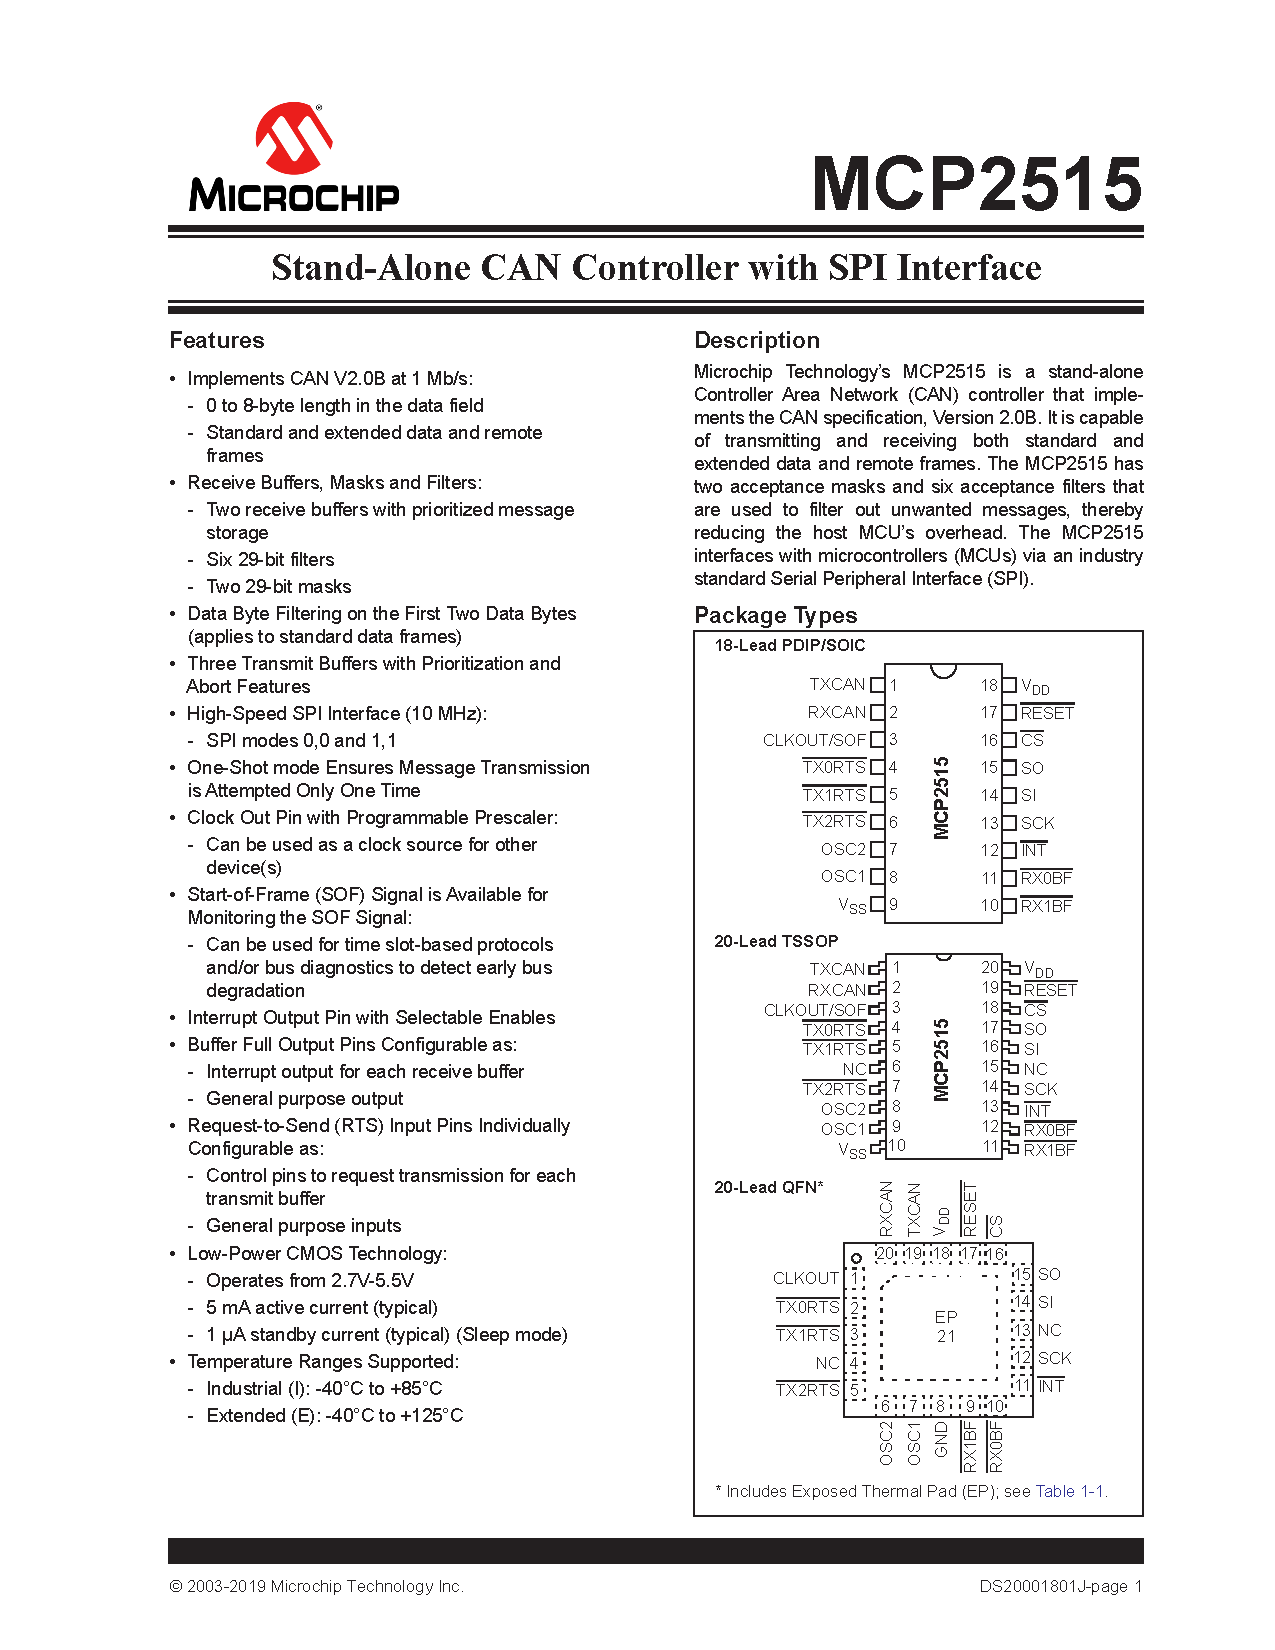
\includegraphics[page=1, width=0.89\textwidth]{DATASHEET/MCP2515.pdf}

	
\end{center}